% ---------------------------------------------------------------
% TCC1 - SENAC SANTO AMARO
% Versão adaptada para o projeto do Matheus
% Tema: classificação de câncer de mama em mamografias
% ---------------------------------------------------------------

\documentclass[
    12pt,
    openright,
    oneside,
    a4paper,
    english,
    brazil
]{abntex2}

% ---------------------------------------------------------------
% PACOTES
% ---------------------------------------------------------------
\usepackage{lmodern}
\usepackage[T1]{fontenc}
\usepackage[utf8]{inputenc}
\usepackage{lastpage}
\usepackage{indentfirst}
\usepackage{color}
\usepackage{graphicx}
\usepackage{microtype}
\usepackage{float}
\usepackage{booktabs}
\usepackage{multirow}
\usepackage{longtable}
\usepackage{amsmath,amssymb}
\usepackage{braket}
\usepackage{pgfgantt}
\usepackage[brazilian,hyperpageref]{backref}
\usepackage[alf]{abntex2cite}
\usepackage[
    left=3cm,
    right=2cm,
    top=3cm,
    bottom=2cm
]{geometry}

% ---------------------------------------------------------------
% CONFIGURAÇÕES DO PDF
% ---------------------------------------------------------------
\makeatletter
\hypersetup{
    pdftitle={\@title},
    pdfauthor={\@author},
    pdfsubject={TCC1 - SENAC Santo Amaro},
    pdfcreator={LaTeX with abnTeX2},
    pdfkeywords={tcc, senac, câncer de mama, cnn, computação quântica},
    colorlinks=true,
    linkcolor=blue,
    citecolor=blue,
    filecolor=magenta,
    urlcolor=blue,
    bookmarksdepth=4
}
\makeatother

\definecolor{blue}{RGB}{41,5,195}

% ---------------------------------------------------------------
% INFORMAÇÕES DO DOCUMENTO
% ---------------------------------------------------------------
\titulo{Classificação de câncer de mama em mamografias: um estudo comparativo entre CNNs clássicas e híbridas quântico-clássicas}
\autor{Matheus Sanchez Duda}
\local{São Paulo}
\data{2026}
\orientador{Prof. Jorge Echeimberg}
\coorientador{Prof. Thyago Quintas}

\instituicao{%
  SENAC -- Serviço Nacional de Aprendizagem Comercial
  \par
  Unidade Santo Amaro
  \par
  Bacharelado em Ciência da Computação
}

\tipotrabalho{Trabalho de Conclusão de Curso I}

\preambulo{Proposta de Trabalho de Conclusão de Curso apresentada ao SENAC Santo Amaro como requisito parcial para aprovação na disciplina de TCC1 do curso de Ciência da Computação.}

\makeindex

\begin{document}
\selectlanguage{brazil}
\frenchspacing

% ---------------------------------------------------------------
% ELEMENTOS PRÉ-TEXTUAIS
% ---------------------------------------------------------------
\pretextual
\imprimircapa
\imprimirfolhaderosto

\begin{resumo}

Este trabalho propõe um estudo comparativo entre redes neurais convolucionais clássicas e modelos híbridos quântico-clássicos aplicados à classificação de câncer de mama em mamografias. A pesquisa parte de experimentos anteriores em três classes diagnósticas (normal, benigna e maligna), nos quais a arquitetura clássica apresentou desempenho médio próximo de 70\%, enquanto o modelo híbrido ainda permaneceu limitado por instabilidade, custo de simulação e desempenho próximo ao acaso. A proposta consiste em estabelecer um protocolo experimental mais robusto, contemplando preparação dos dados, tratamento do desbalanceamento, definição de baselines clássicos, construção de circuitos quânticos simulados e avaliação por métricas preditivas e computacionais. Busca-se verificar se a inclusão de um componente quântico variacional pode produzir comportamento competitivo em relação a alternativas clássicas equivalentes, sem pressupor vantagem quântica e considerando as restrições atuais de número de qubits, profundidade dos circuitos, tempo de simulação e estabilidade do treinamento. O trabalho não tem finalidade diagnóstica clínica, mas contribui para a análise experimental da viabilidade de arquiteturas híbridas em problemas de visão computacional médica.

\vspace{\onelineskip}
\noindent
\textbf{Palavras-chave}: câncer de mama. mamografia. redes neurais convolucionais. computação quântica. aprendizado de máquina quântico.
\end{resumo}

\pdfbookmark[0]{\contentsname}{toc}
\tableofcontents*
\cleardoublepage

% ---------------------------------------------------------------
% ELEMENTOS TEXTUAIS
% ---------------------------------------------------------------
\textual


% ---------------------------------------------------------------
% CAPÍTULO 1 - INTRODUÇÃO
% ---------------------------------------------------------------

\chapter{Introdução}

O avanço da Inteligência Artificial tem ampliado o uso de métodos computacionais em problemas complexos da área da saúde, especialmente em tarefas relacionadas à análise de imagens médicas. Entre essas aplicações, a classificação de mamografias possui relevância social e científica por estar associada ao apoio à identificação de alterações relacionadas ao câncer de mama.

As redes neurais convolucionais consolidaram-se como uma das principais abordagens em visão computacional, pois aprendem padrões visuais diretamente a partir das imagens. Apesar dos avanços obtidos por modelos clássicos de aprendizado profundo, persistem desafios relevantes em aplicações médicas, como generalização entre bases de dados, desbalanceamento de classes, custo computacional, qualidade dos rótulos e confiabilidade dos resultados.

Paralelamente, a computação quântica e o aprendizado de máquina quântico têm despertado interesse como áreas emergentes de pesquisa. Modelos híbridos quântico-clássicos combinam etapas clássicas de processamento com circuitos quânticos parametrizados, buscando explorar novas formas de representação da informação. No entanto, sua aplicação em problemas de alta dimensionalidade, como imagens de mamografia, ainda é limitada e exige avaliação experimental cuidadosa.

Diante desse cenário, este trabalho propõe comparar uma arquitetura clássica baseada em redes neurais convolucionais com uma arquitetura híbrida quântico-clássica aplicada à classificação de mamografias digitais. A comparação considera não apenas desempenho preditivo, mas também estabilidade experimental, custo computacional e viabilidade prática em ambiente de simulação.

Assim, este capítulo apresenta o contexto da pesquisa, o problema investigado, a justificativa, os objetivos, a hipótese e as delimitações do trabalho.

\section{Contexto}

O câncer de mama é uma das doenças oncológicas de maior impacto na saúde pública, tanto por sua elevada incidência quanto pelas consequências clínicas, sociais e econômicas associadas ao diagnóstico e ao tratamento. A detecção precoce é um fator essencial para ampliar as possibilidades de intervenção em estágios iniciais e melhorar o prognóstico das pacientes. Nesse cenário, a mamografia consolidou-se como uma das principais ferramentas de rastreamento, pois permite identificar alterações suspeitas no tecido mamário antes do surgimento de sintomas clínicos evidentes.

Apesar de sua importância, a interpretação de mamografias é uma tarefa complexa. O exame pode apresentar achados sutis, como massas, microcalcificações, assimetrias e distorções arquiteturais, que nem sempre são facilmente distinguíveis do tecido mamário normal. Além disso, fatores como densidade mamária, qualidade da aquisição, variação entre equipamentos, diferenças anatômicas entre pacientes e alto volume de exames analisados por especialistas tornam a leitura mamográfica um processo desafiador.

Nesse contexto, técnicas de Inteligência Artificial têm sido investigadas como ferramentas de apoio à análise de imagens médicas. Entre elas, as redes neurais convolucionais destacam-se por extrair automaticamente padrões espaciais das imagens, sendo amplamente utilizadas em tarefas de classificação, detecção e segmentação. Em mamografias, esses modelos podem auxiliar na identificação de padrões associados a exames normais, alterações benignas e achados malignos, contribuindo para estudos voltados ao apoio computacional à decisão médica.

Ao mesmo tempo, a computação quântica passou a ser investigada como alternativa emergente para problemas de aprendizado de máquina. No campo do Aprendizado de Máquina Quântico, modelos híbridos quântico-clássicos combinam processamento clássico com circuitos quânticos parametrizados, buscando explorar novas formas de representação e transformação da informação. Entretanto, essas abordagens ainda estão em estágio exploratório, especialmente em aplicações com imagens médicas de alta dimensão.

Dessa forma, este trabalho está inserido na interseção entre visão computacional médica, aprendizado profundo e aprendizado de máquina quântico. A pesquisa propõe investigar a classificação de câncer de mama em mamografias por meio de uma comparação controlada entre redes neurais convolucionais clássicas e arquiteturas híbridas quântico-clássicas, considerando métricas preditivas, custo computacional, estabilidade e limitações práticas de simulação.


\section{Problema de pesquisa}

Embora redes neurais convolucionais clássicas já apresentem resultados relevantes em tarefas de classificação de mamografias, ainda existem desafios relacionados à generalização, ao desbalanceamento das bases de dados, à qualidade dos rótulos, ao custo computacional e à confiabilidade dos modelos em cenários experimentais controlados. Em imagens médicas, esses desafios tornam-se mais sensíveis porque pequenas regiões da imagem podem conter informações clinicamente importantes, e erros de classificação podem afetar a interpretação do exame.

Ao mesmo tempo, modelos híbridos quântico-clássicos vêm sendo investigados como alternativa exploratória para tarefas de aprendizado de máquina, com a proposta de representar dados por meio de circuitos quânticos parametrizados. Entretanto, muitos estudos nessa área ainda são realizados em bases pequenas, imagens de baixa resolução, tarefas simplificadas ou ambientes fortemente simulados, o que dificulta avaliar sua viabilidade prática em problemas de maior dimensionalidade, como mamografias.

O problema central deste trabalho está na necessidade de uma comparação controlada entre uma CNN clássica, uma CNN com gargalo clássico e uma arquitetura híbrida quântico-clássica aplicada à classificação de mamografias sob o mesmo protocolo experimental. Sem esse controle, torna-se difícil identificar se a inclusão de um componente quântico contribui de fato para o desempenho do modelo ou se apenas aumenta a complexidade computacional sem trazer ganhos relevantes.

Assim, a pergunta que orienta a pesquisa é: modelos híbridos quântico-clássicos simulados podem apresentar desempenho, estabilidade e viabilidade computacional competitivos em relação a baselines clássicos na classificação de mamografias digitais?

\section{Justificativa}

A justificativa deste trabalho pode ser compreendida em três dimensões. A primeira é a relevância social do tema. O câncer de mama possui alta incidência e depende fortemente de estratégias de detecção precoce e apoio à decisão clínica, o que torna pertinente investigar métodos computacionais capazes de auxiliar a análise de mamografias \cite{WHO2026BreastCancer}. Embora o presente trabalho não tenha objetivo de uso clínico imediato, ele se insere em uma linha de pesquisa com impacto potencial na área da saúde.

A segunda dimensão é a relevância acadêmica. O aprendizado profundo consolidou-se como uma abordagem central em visão computacional, mas a adoção de modelos híbridos quântico-clássicos ainda carece de validação comparativa rigorosa, principalmente em aplicações médicas \cite{LeCun2015,Gupta2025QMLDigitalHealth}. Assim, o TCC contribui ao investigar se a integração de componentes quânticos traz benefícios mensuráveis em um problema concreto e de alta relevância.

A terceira dimensão é a lacuna científica identificada. Estudos sobre deep learning em mamografia apontam desempenho promissor, porém também evidenciam limitações de reprodutibilidade e de avaliação em condições realistas \cite{Bhalla2023MammographyReview}. Na direção quântica, trabalhos recentes mostram resultados competitivos em tarefas de classificação de imagens, mas ainda em cenários restritos, com bases menores, forte dependência de simulação e poucas evidências em contextos próximos do uso aplicado \cite{long2025qcqcnn}. Dessa forma, este TCC busca preencher uma lacuna ao propor uma comparação experimental controlada, reprodutível e metodologicamente explícita entre abordagens clássicas e híbridas no domínio da mamografia.

\section{Objetivo geral}

Investigar comparativamente o desempenho de CNNs clássicas e modelos híbridos quântico-clássicos na classificação de câncer de mama em mamografias, considerando métricas de desempenho preditivo, custo computacional, estabilidade experimental e viabilidade prática, com base inicial em um cenário de três classes e possibilidade de ampliação para classificações mais detalhadas.


\section{Objetivos específicos}

\begin{enumerate} 
    \item Definir a base de dados e as classes diagnósticas utilizadas no experimento;
    \item Preparar um protocolo padronizado de pré-processamento, divisão dos dados, treinamento, validação e teste;
    \item Aprimorar uma CNN clássica para servir como modelo de referência;
    \item Projetar uma arquitetura híbrida quântico-clássica compatível com as limitações de simulação disponíveis;
    \item Investigar configurações do modelo híbrido, como número de qubits, feature map, profundidade do circuito e estratégia de codificação;
    \item Comparar os modelos por meio de métricas preditivas, métricas computacionais e parâmetros associados ao componente quântico, como número de qubits, profundidade do circuito, estratégia de codificação, número de \textit{shots} e tempo de simulação;
    \item Avaliar tempo de treinamento, uso de memória, estabilidade entre execuções e limitações de escalabilidade;
    \item Discutir criticamente as vantagens, limitações e condições de viabilidade da abordagem híbrida quântico-clássica.
\end{enumerate}

\section{Hipótese}

Parte-se da hipótese de que uma arquitetura híbrida quântico-clássica, utilizando circuitos quânticos simulados como componente treinável complementar às camadas clássicas de uma rede neural, pode apresentar desempenho competitivo em relação a baselines clássicos na tarefa de classificação de mamografias. Essa comparação será realizada sob um protocolo experimental controlado, utilizando a mesma base de dados, critérios equivalentes de pré-processamento, divisão dos dados, métricas de avaliação e execução no mesmo ambiente computacional.

No entanto, não se pressupõe superioridade geral da abordagem quântica. Considerando as limitações atuais da computação quântica e da simulação de circuitos quânticos, espera-se que a viabilidade prática dos modelos híbridos seja condicionada por fatores como custo computacional, número reduzido de qubits, sensibilidade a hiperparâmetros, estratégia de codificação dos dados clássicos em estados quânticos e restrições típicas de dispositivos NISQ. Assim, a hipótese central do trabalho não é demonstrar vantagem quântica definitiva, mas investigar em quais condições a abordagem híbrida pode ser competitiva, limitada ou inviável em comparação com modelos clássicos de aprendizado profundo.

\section{Delimitações do trabalho}

Este trabalho será delimitado como um estudo experimental comparativo em visão computacional. A tarefa será formulada como classificação supervisionada de imagens de mamografia, inicialmente em três classes: normal, benigno e maligno. A comparação será realizada entre uma CNN clássica, uma CNN com gargalo clássico e uma arquitetura híbrida quântico-clássica, mantendo-se constantes a base de dados, o pré-processamento, os critérios de divisão dos dados e as métricas de avaliação.

O estudo não pretende propor um sistema de diagnóstico clínico, substituir a avaliação médica ou validar um modelo em ambiente hospitalar. Os circuitos quânticos serão avaliados por simulação clássica, com número reduzido de qubits e profundidade limitada. A eventual ampliação do número de classes dependerá da disponibilidade e da consistência dos rótulos presentes na base utilizada.

% ---------------------------------------------------------------
% CAPÍTULO 2 - REVISÃO BIBLIOGRÁFICA
% ---------------------------------------------------------------
\chapter{Revisão Bibliográfica}

\section{Metodologia da pesquisa bibliográfica}

A pesquisa bibliográfica deste trabalho será conduzida com o objetivo de fundamentar teoricamente e metodologicamente o estudo comparativo entre redes neurais convolucionais clássicas e modelos híbridos quântico-clássicos aplicados à classificação de câncer de mama em imagens de mamografia. A revisão terá caráter narrativo e crítico, pois o objetivo não é apenas listar publicações, mas identificar quais conceitos, métodos, bases de dados, métricas e limitações sustentam a proposta experimental do TCC.

O recorte temporal principal adotado será de 2021 a 2026, priorizando estudos recentes sobre mamografia, aprendizado profundo, validação de modelos em imagens médicas e aprendizado de máquina quântico. Esse recorte é adequado porque o tema envolve tecnologias em rápida evolução, especialmente no uso de arquiteturas híbridas quântico-clássicas e em benchmarks recentes de mamografia. No entanto, o critério temporal não será aplicado de forma rígida quando trabalhos anteriores forem necessários para a fundamentação do problema. Assim, serão incluídas referências seminais ou estruturantes anteriores a 2021 quando elas explicarem conceitos indispensáveis ao trabalho, como redes neurais profundas \cite{LeCun2015,goodfellow2016deep}, arquiteturas convolucionais modernas \cite{he2016resnet}, Grad-CAM \cite{selvaraju2020gradcam}, métricas de classificação \cite{fawcett2006roc,hand2001simple}, fundamentos de computação quântica \cite{nielsen2010quantum,preskill2018nisq} e bases públicas clássicas de mamografia \cite{moreira2012inbreast,lee2017cbisddsm}.

Também serão considerados preprints e pré-publicações recentes, especialmente de arXiv, medRxiv e bioRxiv, quando apresentarem contribuição diretamente relacionada a pontos ainda em consolidação na literatura, como novos benchmarks, estratégias de codificação quântica, simulação de circuitos, otimização de modelos híbridos ou propostas recentes de avaliação em mamografia. Esses trabalhos serão utilizados com cautela: não serão tratados como evidência definitiva quando ainda não tiverem revisão por pares, mas poderão apoiar a discussão de tendências emergentes, escolhas experimentais e limitações técnicas. Nesses casos, a condição de pré-publicação será considerada na análise crítica da confiabilidade do estudo.

As buscas serão realizadas em bases científicas nacionais e internacionais, incluindo Google Scholar, PubMed, IEEE Xplore, ACM Digital Library, Scopus, SciELO e Periódicos CAPES. A escolha dessas bases se justifica pela abrangência de publicações nas áreas de Ciência da Computação, Inteligência Artificial, visão computacional, imagens médicas, radiologia e computação quântica. Também serão consultadas as listas de referências dos artigos selecionados, quando necessário, para localizar trabalhos fundamentais que não se enquadrem no recorte temporal principal, mas sejam recorrentes ou metodologicamente indispensáveis.

Serão utilizadas palavras-chave em português e inglês, combinadas por meio de operadores booleanos. Entre os principais termos estão: \textit{``câncer de mama''}, \textit{``mamografia''}, \textit{``classificação de imagens médicas''}, \textit{``redes neurais convolucionais''}, \textit{``aprendizado profundo''}, \textit{``computação quântica''}, \textit{``aprendizado de máquina quântico''}, \textit{``modelos híbridos quântico-clássicos''}, \textit{``breast cancer''}, \textit{``mammography''}, \textit{``mammogram''}, \textit{``convolutional neural network''}, \textit{``deep learning''}, \textit{``medical image classification''}, \textit{``quantum machine learning''}, \textit{``quantum neural network''}, \textit{``variational quantum circuit''}, \textit{``quantum feature map''}, \textit{``barren plateau''}, \textit{``hybrid quantum-classical neural network''} e \textit{``quantum medical image classification''}.

As strings de busca serão organizadas em blocos temáticos. O primeiro bloco contemplará estudos sobre classificação de câncer de mama em mamografias com redes neurais convolucionais e aprendizado profundo. O segundo abordará detecção, segmentação, regiões de interesse, microcalcificações e massas mamárias. O terceiro tratará de bases de dados e benchmarks públicos de mamografia, como DDSM, CBIS-DDSM, INbreast, CMMD, VinDr-Mammo, CDD-CESM, DMID, RSNA e Mammo-Bench. O quarto bloco reunirá estudos sobre robustez, validação externa, generalização e reprodutibilidade de modelos de aprendizado profundo em mamografia. O quinto bloco contemplará artigos relacionados à explicabilidade, Grad-CAM, aprendizado baseado em patches, \textit{curriculum learning} e uso de anotações fracas ou fortes. Por fim, o sexto bloco reunirá trabalhos sobre aprendizado de máquina quântico, redes neurais quânticas, classificadores variacionais, métodos de kernel quântico, \textit{feature maps}, ansatzes, simulação quântica e arquiteturas híbridas quântico-clássicas.

Como critérios de inclusão, serão selecionados trabalhos em português ou inglês que abordem diretamente pelo menos um dos seguintes pontos: classificação de câncer de mama em mamografias; uso de CNNs ou aprendizado profundo em imagens médicas; bases de dados, benchmarks ou protocolos de validação em mamografia; métricas relevantes para classificação multiclasse e bases desbalanceadas; explicabilidade em redes neurais; fundamentos de computação quântica; aprendizado de máquina quântico; ou modelos híbridos quântico-clássicos aplicados a tarefas de classificação. Serão excluídos trabalhos sem relação direta com imagens médicas, estudos puramente clínicos sem contribuição computacional para o escopo do TCC, publicações sem descrição mínima de método ou métrica, materiais duplicados, textos sem acesso suficiente ao conteúdo metodológico e estudos cujo foco esteja distante da comparação experimental proposta.

A seleção dos artigos será realizada por meio de um funil de busca e triagem, conforme a Figura~\ref{fig:funil_busca_bibliografica}. Inicialmente, serão identificadas publicações nas bases científicas e em repositórios de pré-publicação. Em seguida, serão removidos registros duplicados e materiais claramente fora do escopo. Na etapa de triagem, serão avaliados título, resumo e palavras-chave. Depois, os textos potencialmente relevantes serão avaliados quanto ao objetivo, base de dados utilizada, tipo de imagem, número de classes, arquitetura proposta, métricas de avaliação, estratégia de validação, resultados obtidos, limitações declaradas e relação direta com a proposta deste TCC. Por fim, serão mantidos os trabalhos que contribuírem para a fundamentação teórica, a definição metodológica ou a análise crítica da comparação entre CNN clássica, CNN com gargalo clássico e modelo híbrido quântico-clássico.

\begin{figure}[H]
    \centering
    \begin{tabular}{p{0.22\textwidth}p{0.68\textwidth}}
        \toprule
        \textbf{Etapa do funil} & \textbf{Critério aplicado} \\
        \midrule
        Identificação & Busca em bases científicas, repositórios de pré-publicação e referências dos artigos selecionados. \\
        Remoção de duplicatas & Exclusão de registros repetidos, versões redundantes e fora do escopo. \\
        Triagem inicial & Leitura de título, resumo e palavras-chave para verificar aderência ao tema do TCC. \\
        Elegibilidade & Leitura do texto completo ou de partes metodológicas relevantes, avaliando base, tarefa, arquitetura, métricas, validação e limitações. \\
        Inclusão final & Seleção de estudos recentes, trabalhos seminais indispensáveis e preprints relevantes para fundamentar ou orientar a proposta experimental. \\
        \bottomrule
    \end{tabular}
    \caption{Funil de busca e seleção dos trabalhos da revisão bibliográfica.}
    \label{fig:funil_busca_bibliografica}
\end{figure}

Os artigos selecionados serão organizados em uma matriz de revisão bibliográfica, contendo informações como ano, autores, tipo de publicação, situação da publicação quando se tratar de preprint, base de dados, método, tarefa abordada, métricas, principais resultados, limitações e relação com a proposta do TCC. Para os trabalhos de aprendizado profundo em mamografia, a análise buscará identificar convergências e divergências relacionadas a desempenho preditivo, uso de bases públicas, tratamento de desbalanceamento, validação externa, explicabilidade, custo computacional e limitações de generalização. Para os modelos quânticos e híbridos quântico-clássicos, serão observados número de qubits, estratégia de codificação, \textit{feature map}, ansatz, simulador ou hardware utilizado, número de \textit{shots}, escalabilidade, custo de simulação e comparação com modelos clássicos.

Dessa forma, a pesquisa bibliográfica não terá apenas a finalidade de reunir referências, mas de posicionar criticamente a proposta deste trabalho. A revisão permitirá justificar a escolha da mamografia como domínio de aplicação, a adoção de CNNs como base clássica de comparação, o uso de uma CNN com gargalo clássico como controle experimental, a investigação de modelos híbridos quântico-clássicos como alternativa exploratória e a necessidade de um protocolo controlado, reprodutível e comparativo para avaliar desempenho, custo computacional, estabilidade e viabilidade prática.

\section{Câncer de mama, mamografia e classificação diagnóstica}

Esta seção apresenta os conceitos médicos necessários para compreender o problema computacional abordado neste trabalho. O objetivo não é aprofundar a discussão clínica sobre oncologia ou radiologia, mas introduzir os principais elementos relacionados ao câncer de mama, ao exame de mamografia e aos rótulos diagnósticos utilizados em bases de dados de imagens médicas.

\subsection{Câncer de mama e importância do diagnóstico precoce}

O câncer de mama é uma das doenças oncológicas de maior impacto na saúde pública, especialmente devido à sua alta incidência e à necessidade de identificação precoce para ampliar as possibilidades de tratamento. O diagnóstico em estágios iniciais pode favorecer intervenções menos agressivas, melhorar o acompanhamento clínico e aumentar as chances de resposta terapêutica.

Nesse contexto, os exames de rastreamento têm papel fundamental, pois permitem identificar alterações suspeitas antes mesmo do surgimento de sintomas evidentes. Entre esses exames, a mamografia se destaca como uma das principais ferramentas utilizadas na detecção de alterações no tecido mamário. Por esse motivo, bases de imagens mamográficas têm sido amplamente utilizadas em pesquisas envolvendo visão computacional, aprendizado profundo e sistemas de apoio ao diagnóstico.

Do ponto de vista computacional, o câncer de mama pode ser investigado a partir de imagens médicas rotuladas, nas quais cada exame ou imagem recebe uma classificação associada à condição observada. Essa abordagem permite formular o problema como uma tarefa de classificação supervisionada, em que um modelo aprende padrões visuais presentes nas imagens e tenta associá-los a categorias diagnósticas, como exames normais, alterações benignas ou alterações malignas.

\subsection{Mamografia e principais achados radiológicos}

A mamografia é um exame de imagem baseado em raios X utilizado para visualizar a estrutura interna da mama. Durante o exame, a mama é comprimida para reduzir a sobreposição dos tecidos e melhorar a qualidade da imagem obtida. As imagens resultantes permitem que radiologistas avaliem a presença de alterações anatômicas e sinais suspeitos que possam indicar lesões benignas ou malignas.

A aquisição da mamografia normalmente envolve diferentes projeções da mama. As duas vistas mais comuns são a craniocaudal (CC), obtida de cima para baixo, e a mediolateral oblíqua (MLO), obtida em uma posição angulada. Essas projeções fornecem informações complementares sobre o tecido mamário e são frequentemente utilizadas em conjunto na prática clínica. Em muitos conjuntos de dados, cada exame pode conter imagens da mama esquerda e direita nessas duas vistas, formando um conjunto de quatro imagens por paciente.

Entre os principais achados avaliados em mamografias estão massas, calcificações, assimetrias e distorções arquiteturais. Massas podem aparecer como regiões mais densas, com diferentes formatos, margens e tamanhos. Calcificações correspondem a pequenos depósitos de cálcio, que podem apresentar padrões benignos ou suspeitos. 

A análise dessas imagens é uma tarefa complexa porque muitas alterações são sutis, ocupam regiões pequenas da imagem ou apresentam baixo contraste em relação ao tecido ao redor. Além disso, a densidade mamária, a qualidade da aquisição, o equipamento utilizado e as características anatômicas de cada paciente podem dificultar a interpretação. Essas características tornam a mamografia um domínio desafiador tanto para especialistas humanos quanto para modelos computacionais.

\subsection{Classificação diagnóstica e BI-RADS}

Do ponto de vista clínico, a classificação diagnóstica busca organizar os exames de acordo com o grau de suspeita ou com a condição observada. Em bases de dados de mamografia, é comum encontrar rótulos como \textit{Normal}, \textit{Benign}, \textit{Suspicious Malignant} e \textit{Malignant}. A classe \textit{Normal} representa exames sem achados relevantes; \textit{Benign} indica alterações não cancerígenas; \textit{Suspicious Malignant} representa casos suspeitos que exigem investigação adicional; e \textit{Malignant} corresponde a achados associados ao câncer de mama.

Além dessas categorias, muitos conjuntos de dados também utilizam o sistema BI-RADS (\textit{Breast Imaging Reporting and Data System}), uma padronização empregada por radiologistas para classificar achados em exames de mama. Esse sistema varia de 0 a 6, incluindo desde exames inconclusivos, que exigem avaliação complementar, até casos com malignidade comprovada por biópsia.

No contexto computacional, esses rótulos podem ser utilizados como classes em tarefas de aprendizado supervisionado. Assim, uma imagem mamográfica passa a ser associada a uma categoria diagnóstica, e o modelo computacional é treinado para aprender relações entre padrões visuais e os rótulos disponíveis. Essa formulação permite construir modelos de classificação capazes de estimar a classe mais provável de uma nova imagem, desde que o treinamento seja realizado com dados rotulados e adequadamente organizados.

Neste trabalho, a classificação diagnóstica é considerada como base para a formulação do problema computacional. Entretanto, a definição exata das classes utilizadas nos experimentos, bem como o tratamento de rótulos ausentes ou categorias pouco representadas, será detalhada posteriormente na proposta metodológica.

\section{Bases de dados em mamografia}

As bases de dados de mamografia são fundamentais para o desenvolvimento, treinamento e avaliação de modelos computacionais aplicados à classificação, detecção e segmentação de câncer de mama. A disponibilidade de conjuntos públicos permite que diferentes pesquisas comparem métodos sob condições semelhantes, além de favorecer a reprodutibilidade científica e a validação de novas arquiteturas.

\subsection{Bases públicas e benchmarks em mamografia}

Entre as bases públicas mais utilizadas na literatura estão DDSM, CBIS-DDSM, INbreast, MIAS, BCDR, CMMD, CDD-CESM, DMID, KAU-BCMD e RSNA Screening Mammography. Cada uma dessas bases possui características próprias em relação ao número de imagens, origem dos exames, formato dos arquivos, tipo de anotação e distribuição das classes.

\begin{figure}[H]
    \centering
    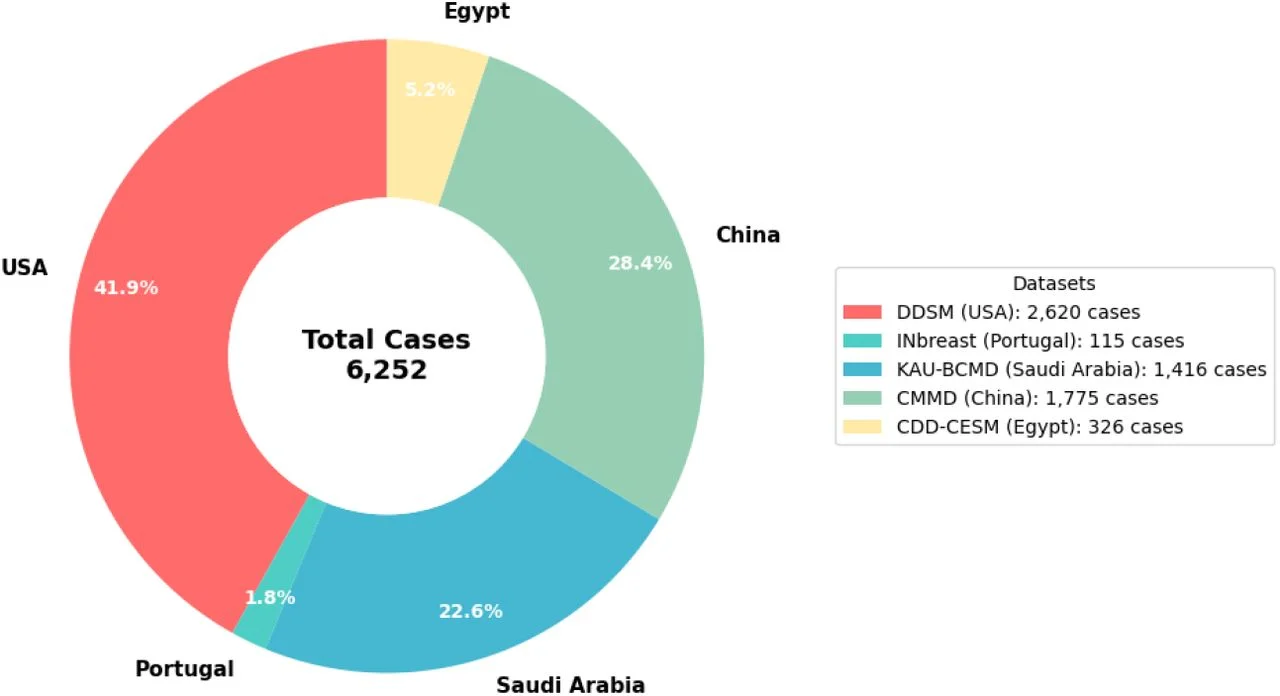
\includegraphics[width=0.85\textwidth]{../figuras/F3.large.png}
    \caption{Distribuição de casos por país e base de origem em parte da composição do Mammo-Bench.}
    \label{fig:representacao-paises-mammobench}
\end{figure}

A Figura~\ref{fig:representacao-paises-mammobench} apresenta a distribuição de casos por país e por base de origem em parte da composição do Mammo-Bench. Observa-se que a maior contribuição vem dos Estados Unidos, representada pela base DDSM, com 2.620 casos, correspondendo a 41,9\% do total apresentado. Em seguida, aparecem a China, por meio da base CMMD, com 1.775 casos (28,4\%), e a Arábia Saudita, representada pela base KAU-BCMD, com 1.416 casos (22,6\%). As menores contribuições são de Egito, com a base CDD-CESM, totalizando 326 casos (5,2\%), e de Portugal, com a base INbreast, contendo 115 casos (1,8\%).

Essa distribuição evidencia que o benchmark reúne dados provenientes de diferentes países e instituições, o que contribui para maior diversidade dos exames mamográficos. Entretanto, também mostra uma concentração relevante em poucas bases, especialmente DDSM, CMMD e KAU-BCMD. Esse aspecto é importante para experimentos de aprendizado de máquina, pois a predominância de determinadas bases pode influenciar o comportamento dos modelos, favorecendo padrões associados a protocolos de aquisição, populações ou formas de anotação mais frequentes no conjunto de dados.

Algumas bases são compostas por mamografias digitalizadas antigas, enquanto outras utilizam mamografias digitais modernas. Também existem diferenças importantes na granularidade das anotações: determinadas bases fornecem regiões de interesse, máscaras ou marcações locais de lesões, enquanto outras disponibilizam apenas rótulos globais por imagem ou por exame. Além disso, metadados como idade da paciente, densidade mamária, BI-RADS, tipo de anormalidade e subtipo molecular nem sempre estão disponíveis em todas as bases.

Essas diferenças impactam diretamente o uso dos dados em aprendizado de máquina. Bases pequenas podem dificultar o treinamento de modelos profundos; bases muito desbalanceadas podem favorecer a classe majoritária; bases coletadas em uma única instituição podem limitar a generalização dos modelos; e a ausência de anotações locais pode restringir experimentos de detecção e segmentação. Por esse motivo, benchmarks que reúnem, padronizam ou organizam diferentes fontes de dados são relevantes para pesquisas comparativas.

Nesse cenário, o Mammo-Bench surge como uma proposta de benchmark de larga escala para mamografias, reunindo diferentes bases públicas em uma estrutura padronizada. Sua composição, organização e distribuição de classes são apresentadas na subseção seguinte, por se tratar da base adotada neste trabalho.

\subsection{Mammo-Bench}

O Mammo-Bench é um conjunto de dados de larga escala voltado para pesquisas em mamografia e classificação de câncer de mama. Ele foi construído a partir da integração de diferentes bases públicas de mamografias, com o objetivo de reunir imagens provenientes de múltiplas fontes, instituições e populações, reduzindo algumas limitações comuns em bases isoladas, como baixo número de amostras, ausência de padronização, diferenças de formato e desbalanceamento entre classes.

Segundo a descrição original do conjunto, o Mammo-Bench reúne imagens mamográficas de 26.500 pacientes provenientes de sete países diferentes, a partir de bases como DDSM, INbreast, KAU-BCMD, CMMD, CDD-CESM, RSNA Screening Dataset e DMID \cite{Bhole2025MammoBench}. Entretanto, na versão dos arquivos CSV analisados neste trabalho, foram encontradas 71.844 imagens, distribuídas entre sete bases de origem. Essa diferença ocorre porque a versão utilizada contém a base \texttt{mini-ddsm}, uma versão reduzida ou filtrada do DDSM original.

As imagens disponibilizadas na versão analisada estão referenciadas em formato \texttt{JPG}. Por se tratar de mamografias, as imagens são tratadas como imagens em escala de cinza, isto é, com apenas um canal de cor. Além disso, os arquivos CSV não informam diretamente as dimensões originais de cada imagem, pois o tamanho final de entrada é definido durante o pré-processamento experimental. Assim, as imagens podem ser redimensionadas conforme a configuração adotada no pipeline de treinamento.

A Tabela~\ref{tab:distribuicao_bases_mammobench} apresenta a distribuição das imagens por base de origem na versão do Mammo-Bench analisada.

\begin{table}[H]
\centering
\caption{Distribuição das imagens por base de origem no CSV do Mammo-Bench}
\label{tab:distribuicao_bases_mammobench}
\begin{tabular}{lrl}
\hline
\textbf{Base no CSV} & \textbf{Quantidade de imagens} & \textbf{Observação} \\ \hline
\texttt{rsna-screening} & 54.705 & Maior base do conjunto; muito desbalanceada \\
\texttt{mini-ddsm}      & 7.808  & Versão reduzida/filtrada do DDSM \\
\texttt{cmmd}           & 5.202  & Subtipo molecular e anormalidades \\
\texttt{kau-bcmd}       & 2.206  & Contém BI-RADS e densidade \\
\texttt{cdd-cesm}       & 1.003  & Mamografia espectral com contraste \\
\texttt{dmid}           & 510    & Pequena, com BI-RADS, densidade e anormalidades \\
\texttt{inbreast}       & 410    & Pequena, mas bem anotada \\ \hline
\textbf{Total}          & \textbf{71.844} & Versão dos CSVs enviados \\ \hline
\end{tabular}
\end{table}

Observa-se que a maior parte das imagens é proveniente da base \texttt{rsna-screening}, que representa 54.705 imagens do total analisado. Essa predominância é relevante do ponto de vista metodológico, pois pode introduzir viés de origem no treinamento dos modelos. Em outras palavras, um modelo pode aprender características associadas à base de dados, ao equipamento ou ao processo de aquisição, em vez de aprender exclusivamente padrões relacionados às alterações mamárias.

Além da diferença na quantidade de imagens por base, o Mammo-Bench também apresenta diferentes tipos de anotação. Entre elas, destacam-se as classes diagnósticas gerais, como \textit{Normal}, \textit{Benign}, \textit{Suspicious Malignant} e \textit{Malignant}; classificações BI-RADS; densidade mamária; tipo de anormalidade; e subtipo molecular, quando disponível. No entanto, nem todas as bases fornecem todos esses tipos de anotação.

No CSV principal, a distribuição das classes diagnósticas por base de origem é apresentada na Tabela~\ref{tab:classes_por_base_mammobench}.


\begin{table}[H]
\centering
\caption{Distribuição das classes por base de origem no CSV principal do Mammo-Bench}
\label{tab:classes_por_base_mammobench}
\resizebox{\textwidth}{!}{%
\begin{tabular}{lrrrrrr}
\hline
\textbf{Base} & \textbf{Normal} & \textbf{Benign} & \textbf{Suspicious Malignant} & \textbf{Malignant} & \textbf{Sem classe} & \textbf{Total} \\ \hline
\texttt{rsna-screening} & 24.021 & 2.265 & 0   & 0     & 28.419 & 54.705 \\
\texttt{mini-ddsm}      & 2.408  & 2.684 & 0   & 2.716 & 0      & 7.808  \\
\texttt{cmmd}           & 0      & 1.108 & 0   & 4.094 & 0      & 5.202  \\
\texttt{kau-bcmd}       & 1.847  & 265   & 72  & 22    & 0      & 2.206  \\
\texttt{cdd-cesm}       & 341    & 331   & 0   & 331   & 0      & 1.003  \\
\texttt{dmid}           & 212    & 154   & 120 & 24    & 0      & 510    \\
\texttt{inbreast}       & 67     & 243   & 43  & 57    & 0      & 410    \\ \hline
\texttt{total-per-class}& 28.896 & 7.050 & 235 & 7.244 & 28.419 & \\
\end{tabular}%
}
\end{table}

A partir da Tabela~\ref{tab:classes_por_base_mammobench}, observa-se que o Mammo-Bench apresenta forte desbalanceamento entre classes e entre bases de origem. A classe \textit{Normal} possui quantidade significativamente maior de imagens em comparação com as classes \textit{Benign} e \textit{Malignant}. Além disso, a base \texttt{rsna-screening} concentra a maior parte das imagens e também apresenta uma quantidade expressiva de registros sem classe diagnóstica definida no CSV principal.

Essas características tornam o Mammo-Bench uma base relevante para estudos de classificação de mamografias, mas também exigem cuidado metodológico em sua utilização. Questões como rótulos ausentes, distribuição desigual entre classes, predominância de determinadas bases de origem e possível viés de aquisição são discutidas na Subseção~\ref{subsec:heterogeneidade_rotulos_limitacoes_bases}.



\subsection{Heterogeneidade, rótulos e limitações das bases de mamografia}
\label{subsec:heterogeneidade_rotulos_limitacoes_bases}

A utilização de bases públicas de mamografia exige atenção à heterogeneidade dos dados. Diferenças entre instituições, equipamentos, protocolos de aquisição, formatos de imagem, critérios de anotação e distribuição das classes podem influenciar diretamente o treinamento e a avaliação de modelos computacionais.

No caso do Mammo-Bench, observa-se a combinação de diferentes bases de origem, com predominância de determinados subconjuntos e presença de rótulos ausentes ou pouco representados. Essas características tornam a base relevante para estudos comparativos, mas também exigem documentação cuidadosa das decisões de filtragem, agrupamento de classes, divisão dos dados e interpretação dos resultados.

Assim, as limitações das bases de mamografia não devem ser tratadas apenas como detalhes de implementação. Elas afetam a validade experimental, a capacidade de generalização e o risco de viés dos modelos. Por isso, questões como qualidade dos rótulos, desbalanceamento, vazamento de dados e métricas por classe serão retomadas na seção de preparação, treinamento e avaliação dos modelos supervisionados.
\section{Inteligência Artificial e aprendizado de máquina}

\subsection{Inteligência Artificial como campo da Ciência da Computação}

A Inteligência Artificial reúne métodos computacionais voltados à construção de sistemas capazes de realizar tarefas que exigem reconhecimento de padrões, tomada de decisão ou inferência a partir de dados. No contexto deste trabalho, o interesse está no uso de técnicas de aprendizado de máquina para classificar imagens de mamografia em categorias diagnósticas.

\subsection{Aprendizado de máquina}

O aprendizado de máquina é uma subárea da Inteligência Artificial na qual modelos computacionais aprendem padrões a partir de exemplos. Em vez de serem programados por regras fixas para cada situação, esses modelos ajustam seus parâmetros com base nos dados disponíveis, buscando produzir previsões adequadas para novas amostras.

\subsection{Aprendizado supervisionado}

No aprendizado supervisionado, cada amostra utilizada no treinamento possui um rótulo conhecido. Assim, o modelo recebe exemplos de entrada e suas respectivas saídas esperadas, aprendendo uma função capaz de associar novas entradas às classes possíveis. Na classificação de mamografias, isso significa associar uma imagem a uma classe diagnóstica, como normal, benigna ou maligna.

\subsection{Representação computacional de imagens digitais}

A classificação computacional de imagens depende da representação de informações visuais em estruturas numéricas manipuláveis por algoritmos. Em processamento digital de imagens, uma imagem pode ser formalmente descrita como uma função bidimensional discreta, composta por elementos finitos denominados pixels, cada um associado a uma posição espacial e a um valor de intensidade \cite{gonzalez2008digital}. No contexto de imagens médicas, especialmente em mamografias, essa representação é fundamental, pois pequenas variações de intensidade, textura e contraste podem indicar estruturas clinicamente relevantes.

Uma imagem digital pode ser compreendida matematicamente como uma função bidimensional discreta, geralmente representada por \(I(x,y)\), em que \(x\) e \(y\) indicam as coordenadas espaciais do pixel e \(I(x,y)\) representa o valor de intensidade naquele ponto da imagem. Em uma imagem em escala de cinza, como ocorre frequentemente em mamografias, cada pixel possui apenas um valor numérico associado à luminosidade local. Assim, uma imagem com altura \(H\) e largura \(W\) pode ser representada como uma matriz:

\[
I \in \mathbb{R}^{H \times W}
\]

A Figura~\ref{fig:imagem_matriz_5x5} apresenta uma representação simplificada dessa estrutura matricial. No exemplo, a imagem em escala de cinza é ampliada como uma grade \(5 \times 5\), na qual cada célula corresponde a um pixel. Ao lado, a mesma imagem é representada por uma matriz de intensidades, em que valores maiores indicam regiões mais claras e valores menores indicam regiões mais escuras.

\begin{figure}[H]
    \centering
    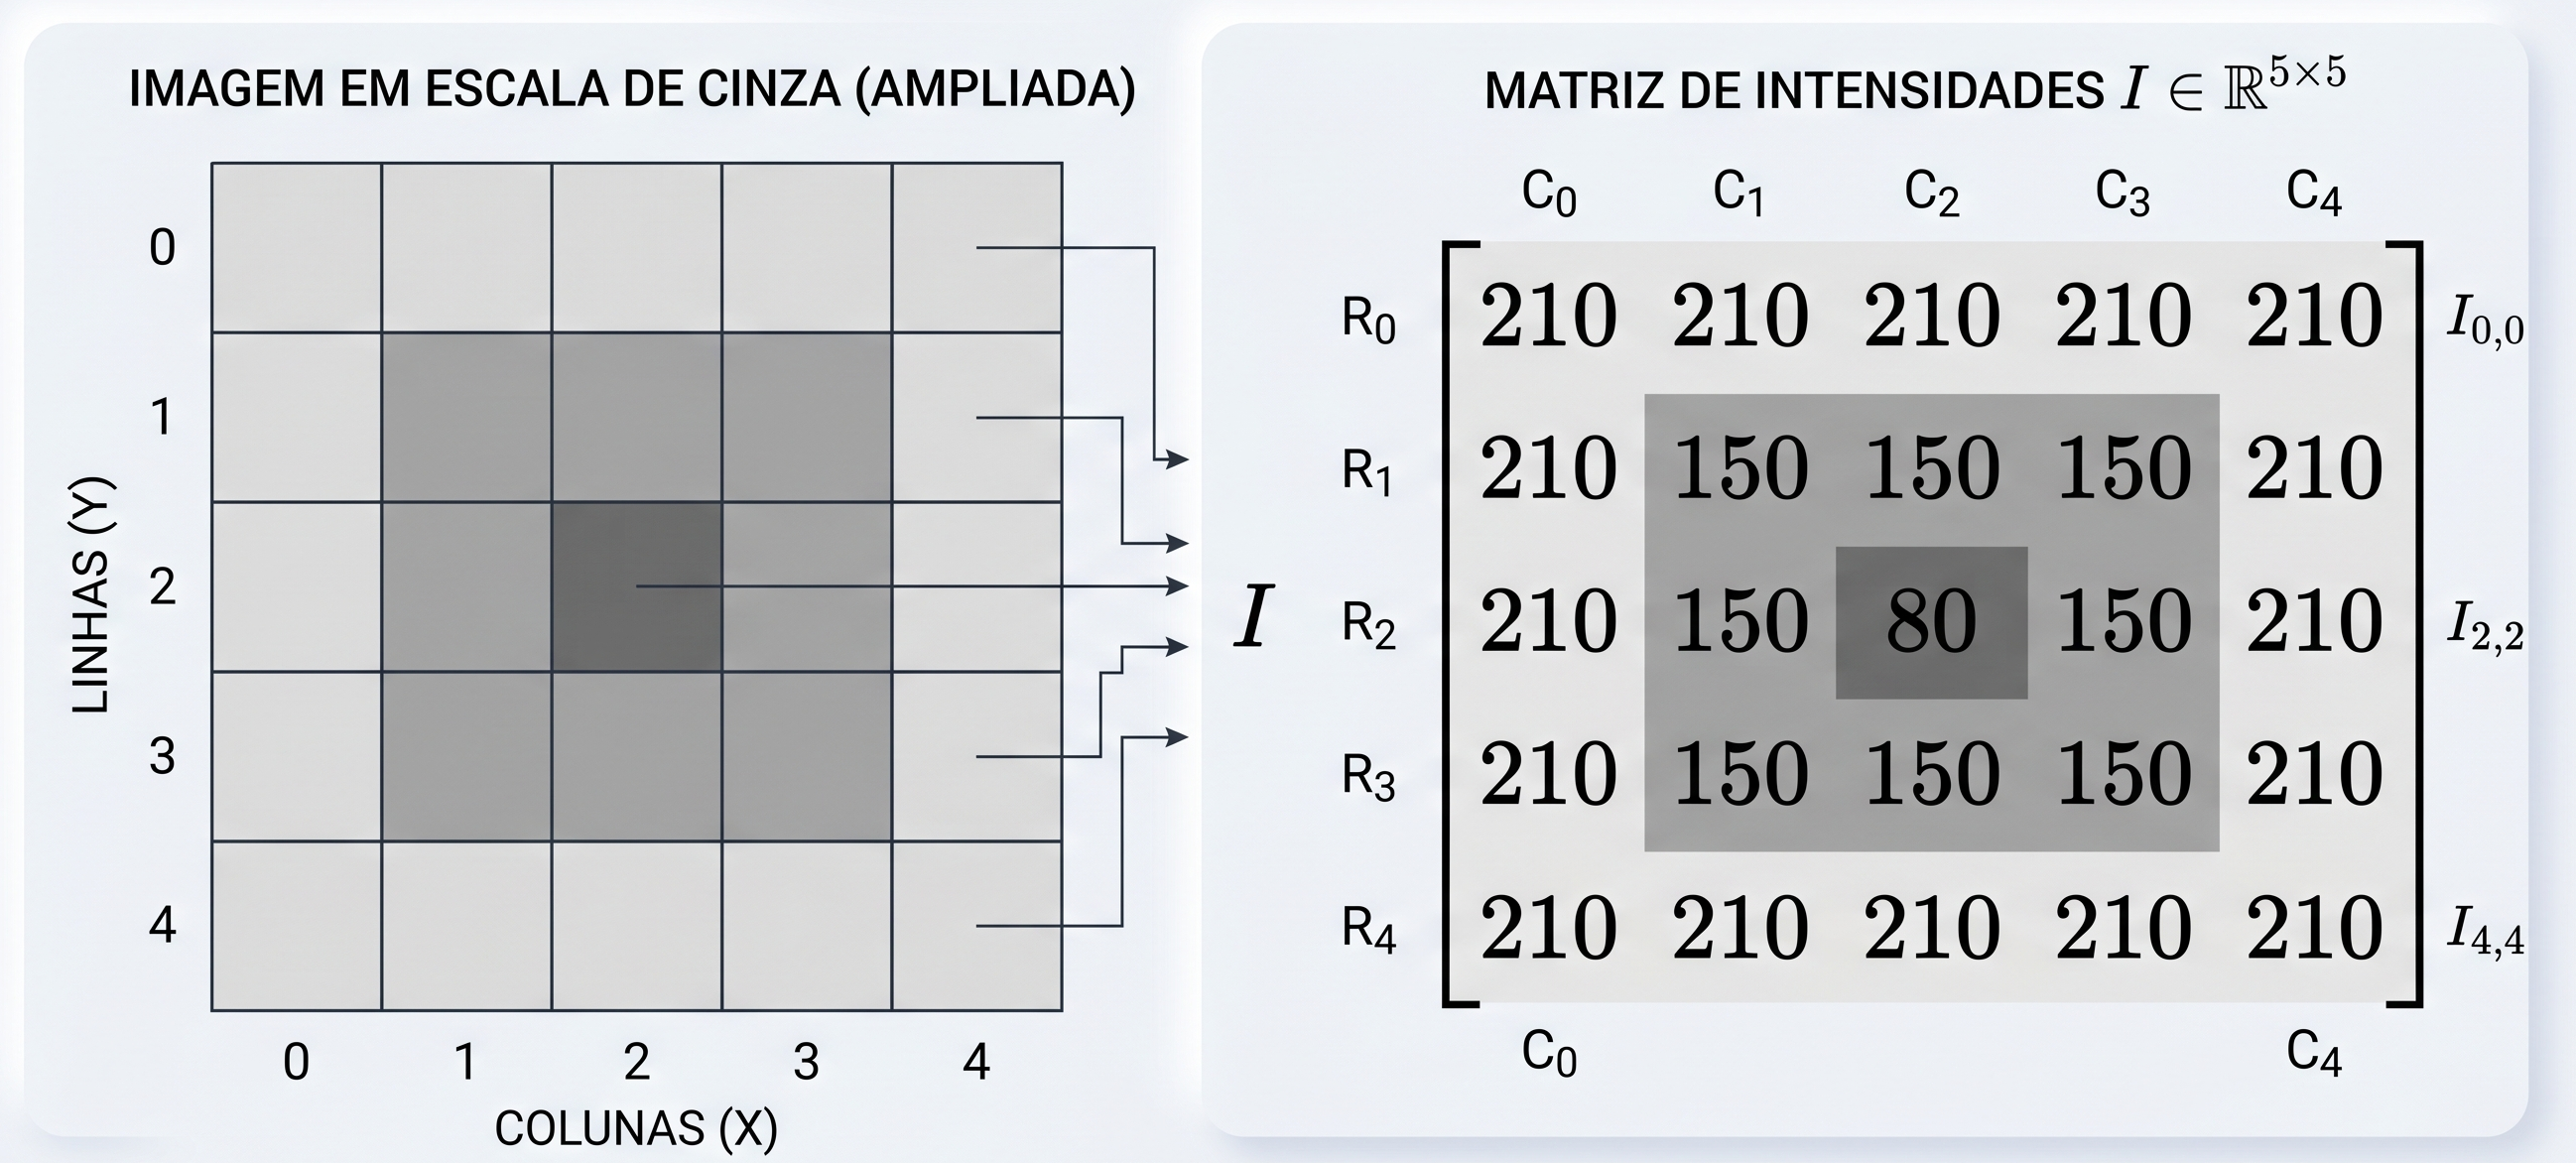
\includegraphics[width=\textwidth]{../figuras/imagem_matriz_5x5.png}
    \caption{Representação matemática de uma imagem em escala de cinza como matriz de intensidades.}
    \label{fig:imagem_matriz_5x5}
\end{figure}

Em termos matemáticos, cada elemento \(I_{i,j}\) corresponde ao valor de intensidade do pixel localizado na linha \(i\) e na coluna \(j\). Em imagens de 8 bits, por exemplo, esses valores normalmente variam entre 0 e 255, sendo 0 associado ao preto, 255 ao branco e os valores intermediários aos diferentes tons de cinza. Em imagens médicas, essa variação de intensidade não representa apenas informação visual, mas também diferenças físicas e anatômicas, como densidade tecidual, contraste entre estruturas e possíveis regiões de interesse clínico.

Antes de ser utilizada por um modelo de aprendizado profundo, a imagem costuma passar por uma etapa de normalização. Uma forma simples de normalização consiste em dividir cada valor de pixel por 255, transformando a escala original para o intervalo entre 0 e 1:

\[
I'_{i,j} = \frac{I_{i,j}}{255}
\]

Essa transformação não altera a estrutura espacial da imagem, mas facilita o treinamento da rede neural, pois reduz a variação numérica dos dados de entrada. Em termos computacionais, uma imagem em escala de cinza também pode ser representada como um tensor de três dimensões:

\[
I \in \mathbb{R}^{H \times W \times C}
\]

em que \(C\) representa o número de canais. No caso de mamografias em escala de cinza, geralmente \(C = 1\). Portanto, uma mamografia redimensionada para \(1024 \times 1024\) pixels pode ser representada como um tensor \(1024 \times 1024 \times 1\). Quando várias imagens são processadas em conjunto durante o treinamento, utiliza-se um lote de imagens, representado por:

\[
X \in \mathbb{R}^{N \times H \times W \times C}
\]

em que \(N\) indica o número de imagens no lote, \(H\) a altura, \(W\) a largura e \(C\) o número de canais.

No contexto da classificação de mamografias, cada imagem \(x\) é associada a um rótulo \(y\), que representa a classe clínica da amostra. Em uma tarefa com três classes, por exemplo, pode-se definir:

\[
y \in \{0, 1, 2\}
\]

em que \(0\) representa uma imagem normal, \(1\) uma imagem benigna e \(2\) uma imagem maligna. O objetivo do modelo computacional é aprender uma função \(f_{\theta}(x)\), parametrizada por pesos treináveis \(\theta\), capaz de receber uma imagem como entrada e produzir uma distribuição de probabilidade sobre as classes possíveis:

\[
f_{\theta}(x) = [p_0, p_1, p_2]
\]

em que \(p_0\), \(p_1\) e \(p_2\) indicam, respectivamente, a probabilidade estimada de a imagem pertencer às classes normal, benigna ou maligna. A classe final prevista pelo modelo é obtida pela escolha da maior probabilidade:

\[
\hat{y} = \arg\max_{k} p_k
\]

Essa formulação mostra que a classificação computacional de imagens não ocorre diretamente sobre a imagem visual percebida por um ser humano, mas sobre uma representação numérica estruturada. A imagem é convertida em matriz ou tensor, seus valores são normalizados, os rótulos são codificados numericamente e o modelo aprende padrões estatísticos capazes de relacionar regiões da imagem às classes de interesse.

Nas redes neurais convolucionais, esse processo é realizado por meio de filtros ou núcleos convolucionais que percorrem a imagem extraindo padrões locais. Um filtro \(K\) de tamanho \(m \times n\) é aplicado sobre pequenas regiões da imagem, produzindo novos mapas de características. De forma simplificada, a operação convolucional pode ser representada por:

\[
S(i,j) = \sum_{u=0}^{m-1}\sum_{v=0}^{n-1} K(u,v) \cdot I(i+u,j+v)
\]

Nesse caso, o filtro funciona como uma janela que analisa regiões locais da imagem. Dependendo dos valores aprendidos pelo filtro durante o treinamento, ele pode se tornar sensível a bordas, texturas, variações de contraste, formas ou padrões mais complexos. Em mamografias, essa propriedade é importante porque alterações clinicamente relevantes podem aparecer como pequenas regiões de maior densidade, massas, microcalcificações ou assimetrias discretas. Assim, a preservação da estrutura espacial da imagem é fundamental para que o modelo consiga aprender relações entre pixels vizinhos e regiões anatômicas relevantes.

Portanto, a representação computacional de imagens digitais é uma etapa central para a classificação automática de mamografias. Ela estabelece a ponte entre a imagem médica original e o modelo de aprendizado profundo, permitindo que informações visuais sejam transformadas em dados numéricos processáveis. Essa base matemática também justifica o uso de redes convolucionais, pois essas arquiteturas exploram diretamente a organização matricial e espacial das imagens.

\subsection{Classificação supervisionada de imagens}
\label{subsec:classificacao_supervisionada_imagens}

A classificação supervisionada de imagens é uma tarefa de aprendizado de máquina na qual um modelo aprende a associar imagens de entrada a rótulos previamente definidos. Diferentemente de abordagens não supervisionadas, nas quais o algoritmo busca padrões sem classes conhecidas, no aprendizado supervisionado cada amostra do conjunto de dados possui uma saída esperada, também chamada de rótulo ou \textit{ground truth}. Em imagens médicas, esses rótulos podem representar categorias diagnósticas, como exame normal, alteração benigna ou alteração maligna.

Do ponto de vista matemático, um conjunto de dados supervisionado pode ser representado por:

\[
\mathcal{D} =
\{(x_1,y_1),(x_2,y_2),\ldots,(x_N,y_N)\},
\]

em que \(x_i\) representa a \(i\)-ésima imagem e \(y_i\) representa seu respectivo rótulo. Em uma tarefa de classificação com \(K\) classes, cada rótulo pertence ao conjunto:

\[
y_i \in \{0,1,\ldots,K-1\}.
\]

Assim, no caso de uma classificação diagnóstica com três classes, pode-se representar os rótulos como \(0\), \(1\) e \(2\), correspondendo, por exemplo, às classes \textit{Normal}, \textit{Benign} e \textit{Malignant}. Essa representação transforma o problema clínico em uma tarefa computacional de classificação multiclasse.

Segundo Deisenroth, Faisal e Ong, a aprendizagem de máquina pode ser compreendida a partir de três componentes principais: dados, modelo e aprendizagem. Os dados precisam ser representados numericamente; o modelo é uma função parametrizada; e a aprendizagem corresponde ao ajuste dos parâmetros desse modelo com base nos exemplos disponíveis \cite{deisenroth2020mathematics}. No caso de imagens digitais, cada imagem pode ser representada como uma matriz ou tensor de valores numéricos. Uma imagem em escala de cinza pode ser descrita como:

\[
x_i \in \mathbb{R}^{H \times W \times C},
\]

em que \(H\) representa a altura, \(W\) representa a largura e \(C\) representa o número de canais. Em mamografias em escala de cinza, normalmente \(C=1\). Dessa forma, a imagem deixa de ser apenas uma informação visual e passa a ser uma estrutura matemática que pode ser processada por algoritmos de aprendizado.

O objetivo de um modelo supervisionado é aprender uma função parametrizada capaz de mapear a entrada \(x_i\) para uma saída associada às classes possíveis. Essa função pode ser representada por:

\[
f_{\theta}: \mathbb{R}^{H \times W \times C} \rightarrow \mathbb{R}^{K},
\]

em que \(\theta\) representa o conjunto de parâmetros aprendidos pelo modelo e \(K\) representa o número de classes. Em redes neurais, esses parâmetros correspondem aos pesos e vieses das camadas. A saída da rede geralmente é um vetor de escores, que pode ser convertido em probabilidades por meio da função \textit{softmax}:

\[
p_k =
\frac{e^{s_k}}
{\sum_{j=0}^{K-1} e^{s_j}},
\]

em que \(s_k\) é o escore associado à classe \(k\), e \(p_k\) representa a probabilidade estimada para essa classe. A classe prevista pelo modelo é dada por:

\[
\hat{y} =
\arg\max_k p_k.
\]

Assim, o modelo atribui à imagem a classe que possui maior probabilidade estimada. Por exemplo, se a saída do modelo para uma mamografia for:

\[
\hat{p} = [0{,}12,\ 0{,}23,\ 0{,}65],
\]

então a classe prevista será a terceira classe, pois \(0{,}65\) é o maior valor do vetor de probabilidades.

Durante o treinamento, a predição do modelo é comparada com o rótulo verdadeiro por meio de uma função de perda. Em problemas multiclasse, uma função frequentemente utilizada é a entropia cruzada categórica:

\[
\mathcal{L}(y,\hat{p}) =
-\sum_{k=0}^{K-1}
y_k \log(p_k),
\]

em que \(y_k\) representa o rótulo verdadeiro em codificação \textit{one-hot}. Quando a classe correta é \(c\), essa expressão pode ser simplificada para:

\[
\mathcal{L}(y,\hat{p}) =
-\log(p_c).
\]

Portanto, a perda será baixa quando o modelo atribuir alta probabilidade à classe correta e será alta quando o modelo atribuir baixa probabilidade ao rótulo verdadeiro. O treinamento consiste em ajustar os parâmetros \(\theta\) para minimizar essa perda ao longo do conjunto de dados, processo diretamente relacionado à otimização matemática em aprendizado de máquina \cite{deisenroth2020mathematics,goodfellow2016deep}.

Em imagens médicas, a classificação supervisionada exige cuidados adicionais. Os rótulos podem apresentar incertezas, inconsistências ou diferenças entre avaliadores; as classes podem ser desbalanceadas; e imagens provenientes de diferentes equipamentos, instituições ou protocolos de aquisição podem apresentar variações importantes. Abdelhafiz et al. destacam que bases de mamografia são fundamentais para treinamento, teste e avaliação de modelos de aprendizado profundo, mas também apresentam diferenças em resolução, formato, tipo de imagem, anotações e distribuição entre classes \cite{abdelhafiz2019}. Essas características tornam a classificação supervisionada de mamografias uma tarefa sensível, na qual o desempenho do modelo depende tanto da arquitetura escolhida quanto da qualidade e organização dos dados.

Além disso, a literatura mostra que CNNs têm sido aplicadas em mamografia para diferentes tarefas, como classificação, detecção de lesões, localização, avaliação de risco e recuperação de imagens \cite{abdelhafiz2019}. Isso reforça que a classificação supervisionada de imagens médicas não se limita ao aprendizado de uma relação matemática entre entrada e saída, mas envolve também a definição adequada do problema clínico, dos rótulos utilizados, da divisão dos dados e das métricas de avaliação.

\section{Aprendizado profundo e redes neurais}

\subsection{Aprendizado profundo}

As redes neurais artificiais fazem parte do campo do aprendizado de máquina, no qual modelos computacionais são treinados para reconhecer padrões a partir de dados. Do ponto de vista matemático, um problema de aprendizado supervisionado pode ser representado por um conjunto de exemplos rotulados:

\[
\mathcal{D} = \{(x_1,y_1),(x_2,y_2),\ldots,(x_N,y_N)\},
\]

em que \(x_i\) representa uma entrada e \(y_i\) representa o rótulo associado a essa entrada. Em uma tarefa de classificação de mamografias, \(x_i\) corresponde a uma imagem mamográfica representada numericamente, enquanto \(y_i\) pertence ao conjunto de classes diagnósticas consideradas.

Segundo Deisenroth, Faisal e Ong, a aprendizagem de máquina pode ser compreendida a partir de três componentes principais: dados, modelo e aprendizagem. Os dados precisam ser convertidos para uma representação numérica; o modelo descreve uma função parametrizada; e a aprendizagem corresponde ao ajuste desses parâmetros a partir dos dados disponíveis, com o objetivo de obter bom desempenho em exemplos ainda não vistos \cite{deisenroth2020mathematics}.

Assim, um modelo de aprendizado profundo pode ser descrito como uma função parametrizada:

\[
f_{\theta}: \mathbb{R}^{D} \rightarrow \mathbb{R}^{K},
\]

em que \(D\) representa a dimensão da entrada, \(K\) representa o número de classes e \(\theta\) representa o conjunto de parâmetros aprendidos pelo modelo. No caso de uma classificação em três classes, como \textit{Normal}, \textit{Benign} e \textit{Malignant}, tem-se \(K=3\).

O aprendizado profundo, ou \textit{deep learning}, diferencia-se de métodos tradicionais por utilizar múltiplas camadas de transformação não linear. Essas camadas permitem que o modelo aprenda representações hierárquicas dos dados. Em imagens, camadas iniciais tendem a capturar padrões simples, como bordas, contrastes e texturas, enquanto camadas mais profundas combinam essas informações em estruturas mais abstratas e semanticamente relevantes.

Esse processo é particularmente importante em imagens médicas, pois as características relevantes nem sempre são evidentes visualmente. Em mamografias, por exemplo, regiões pequenas e de baixo contraste podem conter informações importantes para diferenciar padrões normais, benignos e malignos. Por isso, redes profundas tornaram-se uma abordagem importante para tarefas de classificação, detecção e segmentação em imagens médicas.

\subsection{Redes neurais artificiais}

Uma rede neural artificial é composta por unidades matemáticas chamadas neurônios artificiais, organizadas em camadas. Cada neurônio recebe um conjunto de entradas, aplica uma combinação linear desses valores e, em seguida, utiliza uma função de ativação não linear. Considerando uma entrada \(x \in \mathbb{R}^{D}\), uma camada densa pode ser representada por:

\[
z = Wx + b,
\]

em que \(W \in \mathbb{R}^{M \times D}\) é a matriz de pesos, \(b \in \mathbb{R}^{M}\) é o vetor de vieses e \(z \in \mathbb{R}^{M}\) é o vetor de ativações antes da aplicação da função não linear. Após a função de ativação \(\phi\), obtém-se:

\[
h = \phi(z) = \phi(Wx + b).
\]

A função de ativação é fundamental porque introduz não linearidade ao modelo. Sem ela, a composição de várias camadas lineares poderia ser reduzida a uma única transformação linear. Com funções como ReLU, sigmoid, tanh ou SiLU, a rede passa a representar relações mais complexas entre entrada e saída.

Em uma rede com múltiplas camadas, a saída de uma camada é utilizada como entrada da camada seguinte. Assim, para uma camada \(l\), tem-se:

\[
h^{(l)} = \phi\left(W^{(l)}h^{(l-1)} + b^{(l)}\right),
\]

em que \(h^{(l-1)}\) representa a saída da camada anterior, \(W^{(l)}\) a matriz de pesos da camada atual e \(b^{(l)}\) o vetor de vieses. O conjunto de todos os pesos e vieses da rede compõe os parâmetros \(\theta\).

Em tarefas de classificação multiclasse, a última camada geralmente produz um vetor de escores \(s \in \mathbb{R}^{K}\), em que cada componente corresponde a uma classe. Para transformar esses escores em probabilidades, utiliza-se a função \textit{softmax}:

\[
p_k =
\frac{e^{s_k}}
{\sum_{j=0}^{K-1} e^{s_j}},
\]

em que \(p_k\) representa a probabilidade estimada para a classe \(k\). A classe prevista é dada por:

\[
\hat{y} = \arg\max_k p_k.
\]

O treinamento da rede consiste em ajustar os parâmetros \(\theta\) para reduzir a diferença entre a saída prevista e o rótulo verdadeiro. Para isso, define-se uma função de perda. Em problemas de classificação multiclasse, uma escolha comum é a entropia cruzada categórica:

\[
\mathcal{L}(y,\hat{p}) =
-\sum_{k=0}^{K-1} y_k \log(p_k),
\]

em que \(y_k\) representa o rótulo verdadeiro em codificação \textit{one-hot}. O objetivo do treinamento pode ser expresso como a minimização do risco empírico:

\[
R_{\text{emp}}(\theta) =
\frac{1}{N}
\sum_{i=1}^{N}
\mathcal{L}(y_i, f_{\theta}(x_i)).
\]

A atualização dos parâmetros é feita por métodos de otimização baseados em gradiente. De forma simplificada, uma etapa de gradiente descendente pode ser escrita como:

\[
\theta_{t+1}
=
\theta_t
-
\eta \nabla_{\theta}R_{\text{emp}}(\theta_t),
\]

em que \(\eta\) é a taxa de aprendizado e \(\nabla_{\theta}R_{\text{emp}}\) representa o gradiente da função de perda em relação aos parâmetros. Esse processo mostra que redes neurais dependem diretamente de fundamentos matemáticos como álgebra linear, cálculo vetorial, probabilidade e otimização \cite{deisenroth2020mathematics}.

O cálculo dos gradientes em redes profundas é realizado por meio da retropropagação do erro, ou \textit{backpropagation}. Esse algoritmo utiliza a regra da cadeia para calcular a contribuição de cada parâmetro para o erro final, permitindo que os pesos sejam atualizados progressivamente durante o treinamento. Assim, a rede aprende uma transformação capaz de mapear entradas numéricas para classes de saída.

\subsection{Redes neurais convolucionais}
\label{subsec:redes_neurais_convolucionais}

As redes neurais convolucionais, ou CNNs (\textit{Convolutional Neural Networks}), são arquiteturas especializadas no processamento de dados com estrutura espacial, como imagens. Diferentemente das redes densas, nas quais todos os neurônios de uma camada se conectam a todos os neurônios da camada seguinte, as CNNs exploram a organização local dos pixels por meio de filtros convolucionais. Essa característica reduz o número de parâmetros, preserva relações espaciais e permite que a rede aprenda padrões visuais relevantes diretamente a partir dos dados.

Em uma imagem digital, pixels vizinhos geralmente possuem relações importantes entre si. Bordas, texturas, contrastes, formas e pequenas estruturas anatômicas não aparecem como valores isolados, mas como padrões distribuídos em regiões locais da imagem. Por esse motivo, as CNNs são especialmente adequadas para tarefas de visão computacional, pois aplicam filtros sobre pequenas janelas da imagem, extraindo informações locais que são combinadas progressivamente ao longo das camadas.

Matematicamente, uma convolução discreta pode ser entendida como a aplicação de um filtro, ou \textit{kernel}, sobre uma imagem. Considerando uma imagem bidimensional \(I\) e um filtro \(K\) de tamanho \((2a+1) \times (2b+1)\), a saída da convolução em uma posição \((i,j)\) pode ser representada por:

\[
S(i,j) =
\sum_{m=-a}^{a}
\sum_{n=-b}^{b}
K(m,n)\cdot I(i+m,j+n).
\]

Nessa expressão, \(I(i+m,j+n)\) representa os pixels vizinhos à posição analisada, enquanto \(K(m,n)\) representa os pesos do filtro. O resultado \(S(i,j)\) corresponde à resposta do filtro naquela região da imagem. Assim, cada posição do mapa de saída resume uma combinação ponderada de uma vizinhança local da imagem original.

A Figura~\ref{fig:convolucao_pooling} apresenta uma representação esquemática da aplicação de um filtro convolucional sobre uma imagem e da etapa posterior de \textit{pooling}. A convolução percorre a imagem por regiões locais e produz um mapa de características; em seguida, o \textit{pooling} reduz a dimensão espacial desse mapa, preservando informações consideradas mais relevantes.

\begin{figure}[H]
    \centering
    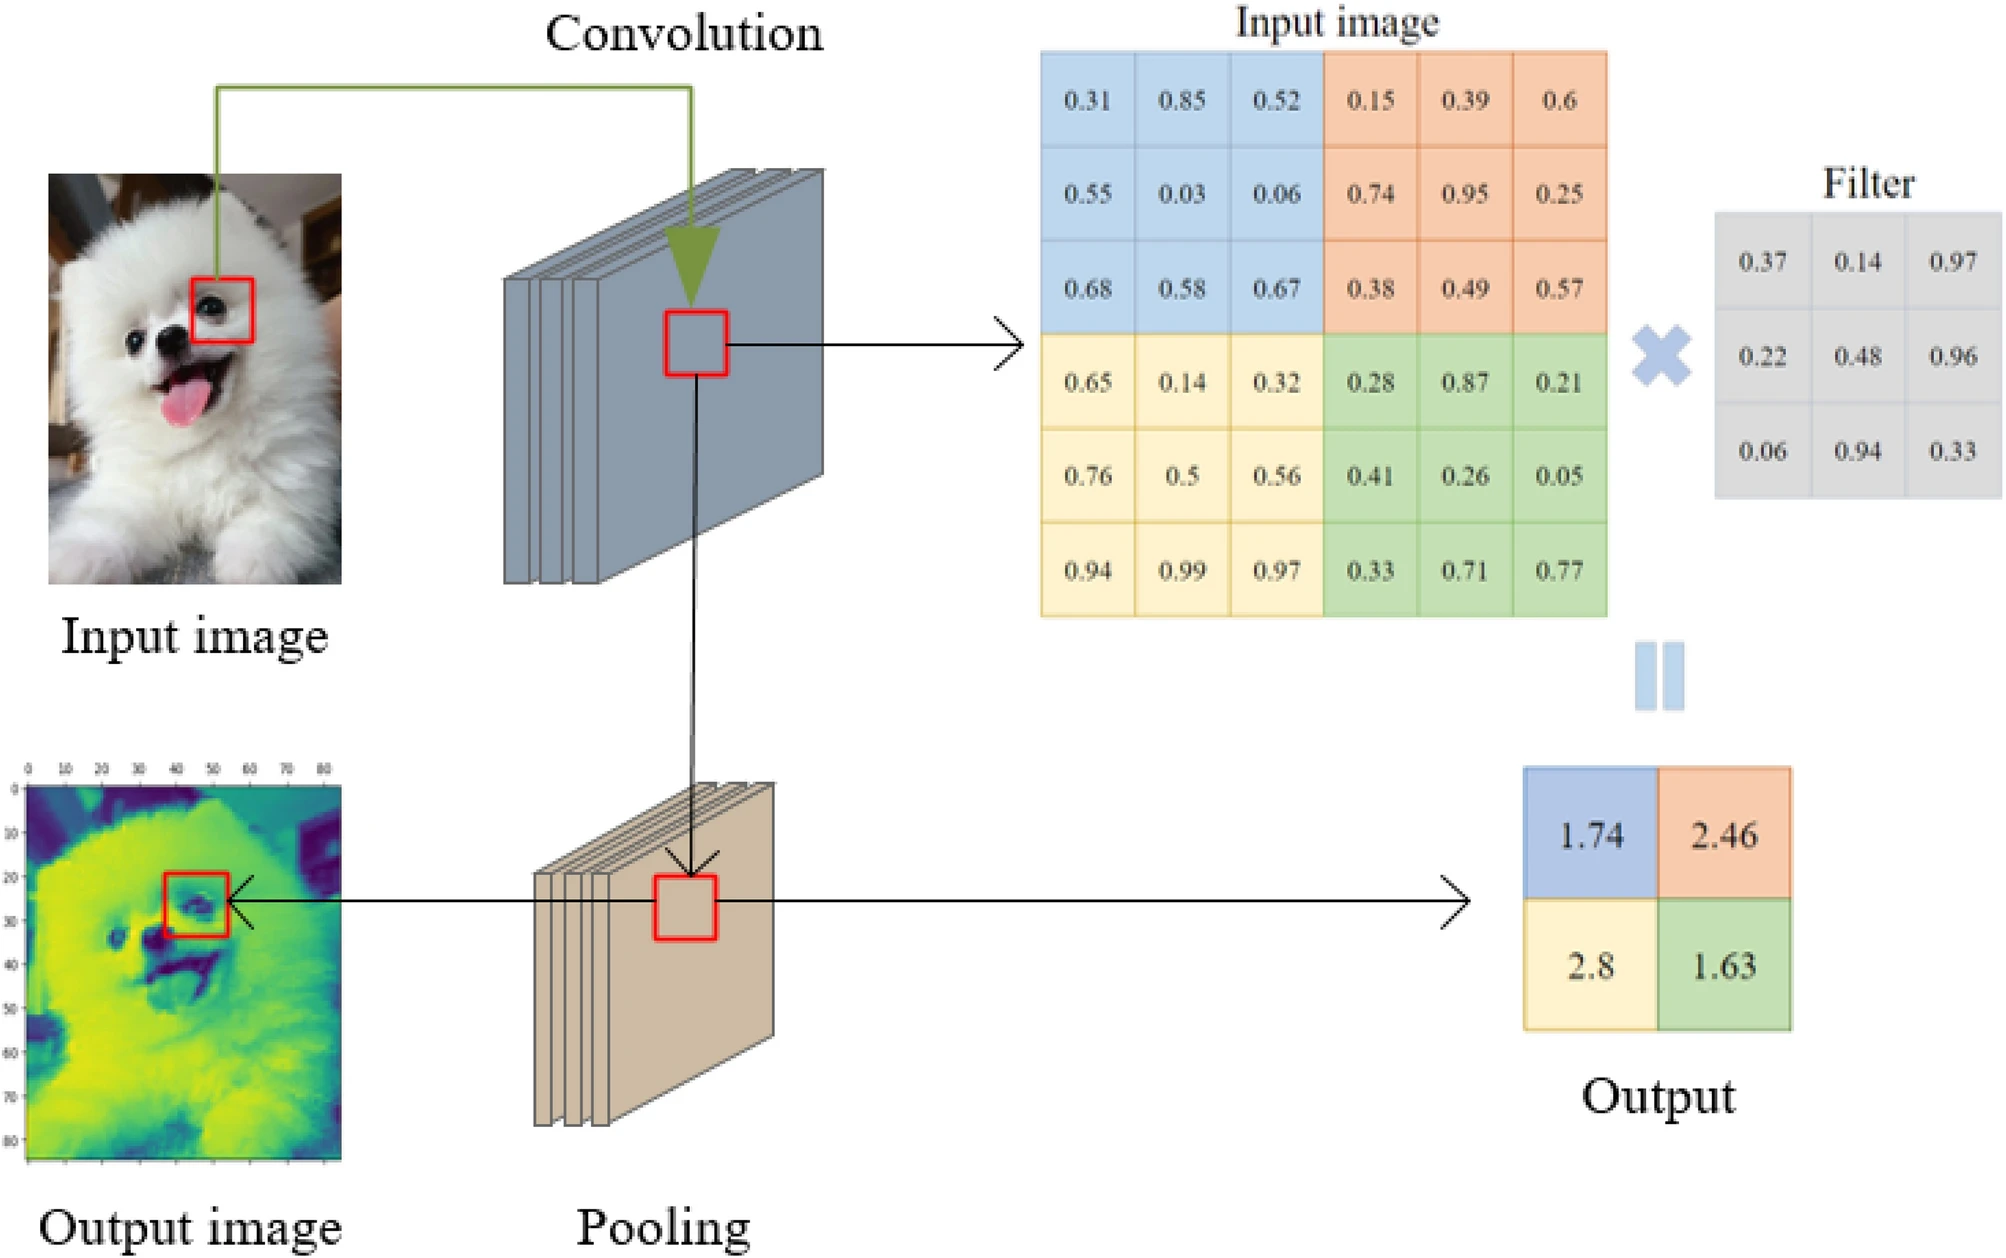
\includegraphics[width=0.85\textwidth]{../figuras/convolutional-pooling.png}
    \caption{Representação esquemática das operações de convolução e \textit{pooling} em uma rede neural convolucional. Fonte: adaptado de Zhao e Zhang \cite{zhao2024improvedpooling}.}
    \label{fig:convolucao_pooling}
\end{figure}

Em uma CNN, os valores dos filtros não são definidos manualmente. Eles são aprendidos durante o treinamento, de acordo com a função de perda e com os dados apresentados à rede. Nas primeiras camadas, os filtros tendem a capturar padrões simples, como bordas, contornos, regiões de contraste e texturas. Nas camadas intermediárias e profundas, esses padrões são combinados em representações mais complexas, capazes de descrever estruturas maiores e mais abstratas.

Em uma camada convolucional, vários filtros são aplicados sobre a imagem ou sobre os mapas de características produzidos pela camada anterior. Cada filtro gera um mapa de características diferente, destacando um tipo de padrão visual. Para uma entrada com múltiplos canais, a saída de um filtro \(r\) pode ser escrita como:

\[
S_r(i,j) =
\sum_{c=1}^{C}
\sum_{m=-a}^{a}
\sum_{n=-b}^{b}
K_{r,c}(m,n)\cdot I_c(i+m,j+n) + b_r,
\]

em que \(C\) é o número de canais de entrada, \(r\) identifica o filtro utilizado, \(K_{r,c}\) representa os pesos do filtro \(r\) aplicados ao canal \(c\), e \(b_r\) é o viés associado ao filtro. Em imagens RGB, por exemplo, \(C=3\). Em mamografias em escala de cinza, geralmente \(C=1\), pois há apenas um canal de intensidade.

Após a convolução, aplica-se normalmente uma função de ativação não linear, como a ReLU (\textit{Rectified Linear Unit}):

\[
ReLU(x) = \max(0,x).
\]

Essa função mantém valores positivos e zera valores negativos, introduzindo não linearidade ao modelo. Sem funções de ativação, a composição de várias camadas convolucionais e densas poderia ser reduzida a uma transformação linear, limitando a capacidade da rede de representar padrões complexos.

Depois da ativação, é comum utilizar uma camada de \textit{pooling}. O \textit{pooling} reduz a dimensão espacial dos mapas de características, diminuindo o custo computacional e tornando a representação mais compacta. Uma operação comum é o \textit{max pooling}, definida por:

\[
P(i,j) =
\max_{(m,n)\in R_{ij}}
S(m,n),
\]

em que \(R_{ij}\) representa uma região local do mapa de características. Nesse caso, a saída corresponde ao maior valor dentro da janela analisada. Também existe o \textit{average pooling}, que calcula a média dos valores da região. Zhao e Zhang \cite{zhao2024improvedpooling} destacam que o \textit{pooling} é importante para reduzir as dimensões espaciais e o volume de dados, mas também pode causar perda de informações, especialmente quando detalhes pequenos são relevantes.

Esse ponto é particularmente importante em imagens médicas. Em mamografias, achados como microcalcificações podem ocupar áreas muito pequenas da imagem. Portanto, embora o \textit{pooling} ajude a reduzir o custo computacional, seu uso deve ser cuidadosamente planejado para evitar a perda de detalhes clinicamente relevantes.

A Figura~\ref{fig:feature_maps} mostra uma visualização de mapas de características produzidos em diferentes blocos convolucionais. Observa-se que as primeiras camadas ainda preservam boa parte da estrutura visual da imagem original, enquanto camadas mais profundas produzem ativações mais abstratas e espacialmente reduzidas. Esse comportamento ilustra a ideia de aprendizado hierárquico em CNNs: padrões simples são aprendidos nas camadas iniciais e combinados em representações mais complexas nas camadas posteriores.

\begin{figure}[H]
    \centering
    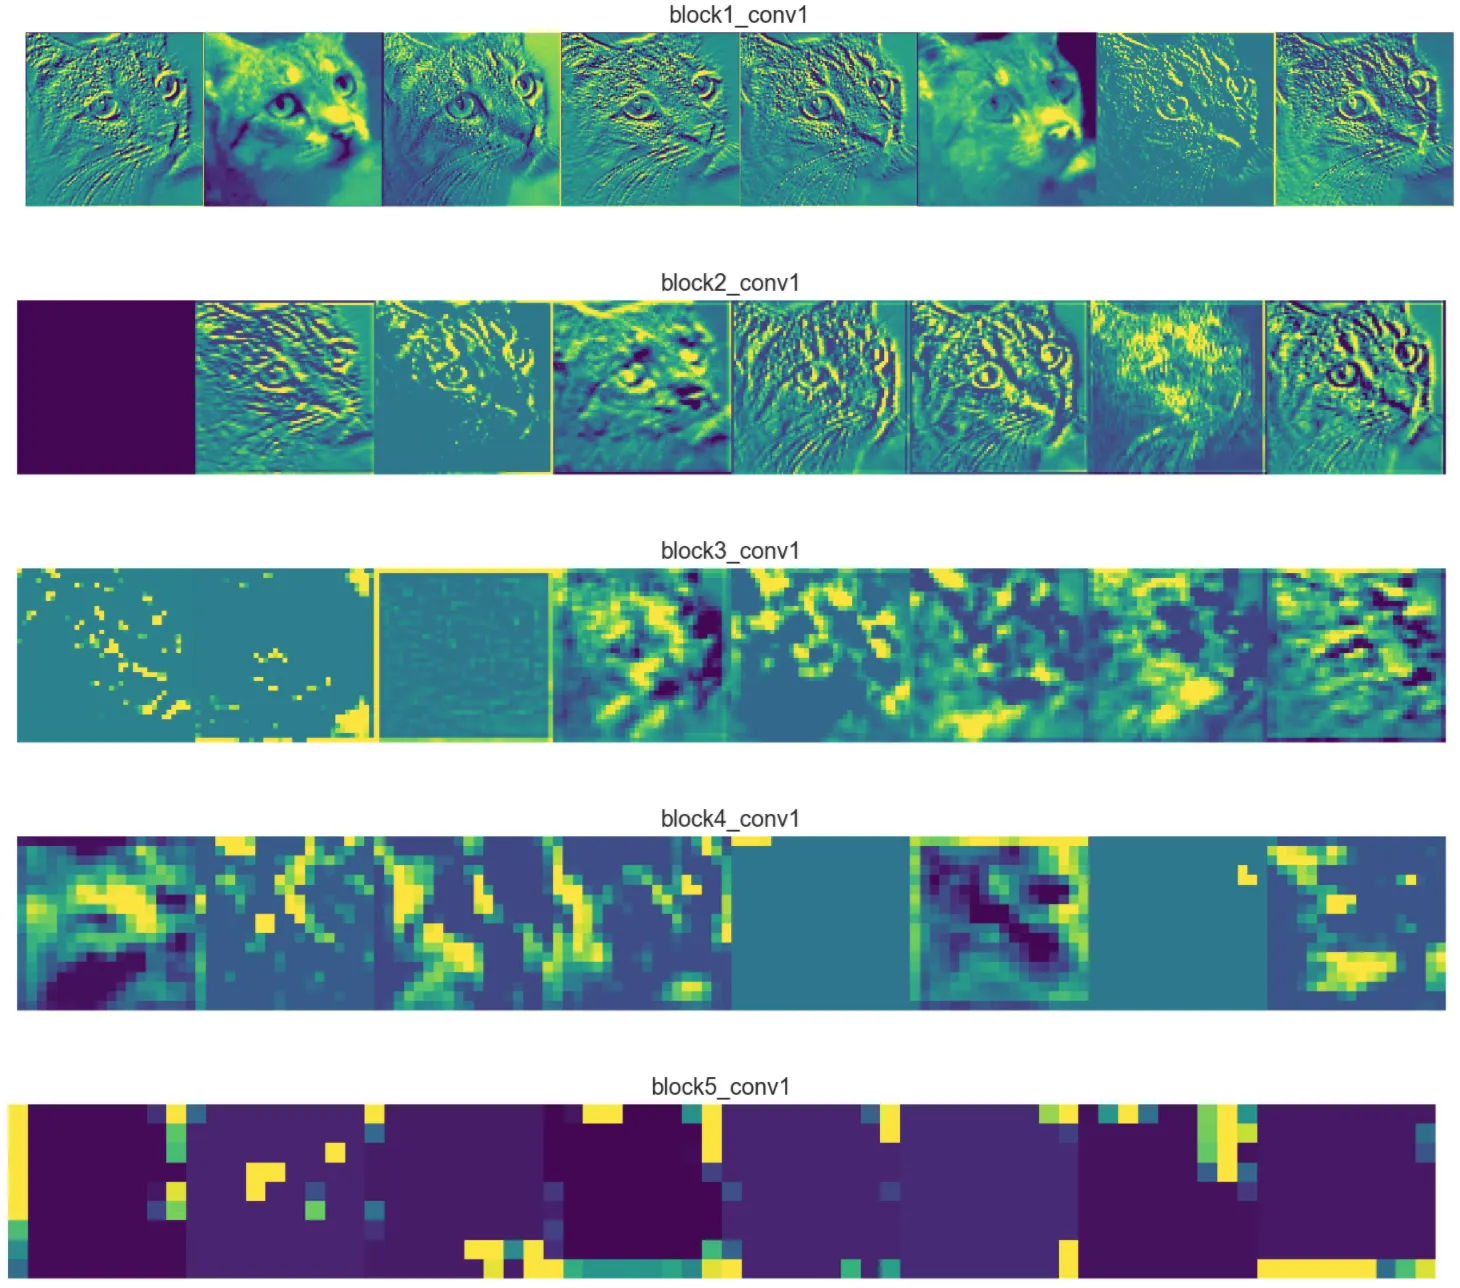
\includegraphics[width=\textwidth]{../figuras/feature-map-converted.png}
    \caption{Exemplo de visualização de mapas de características em diferentes blocos convolucionais. As camadas iniciais tendem a preservar bordas, texturas e contornos, enquanto camadas mais profundas representam padrões mais abstratos. Fonte: adaptado de Hesaraki \cite{hesaraki2023featuremap}.}
    \label{fig:feature_maps}
\end{figure}

O desenvolvimento das CNNs profundas foi fundamental para o avanço da visão computacional. Arquiteturas como AlexNet, VGG, GoogLeNet/Inception e ResNet demonstraram que redes convolucionais profundas podem aprender representações hierárquicas altamente eficazes para classificação de imagens. Szegedy et al. propuseram a arquitetura GoogLeNet/Inception, mostrando que é possível aumentar profundidade e largura da rede mantendo preocupação com eficiência computacional \cite{szegedy2014going}. Essa preocupação também é relevante em imagens médicas, nas quais a resolução das imagens pode ser alta e o custo de processamento tende a ser elevado.

A Figura~\ref{fig:convolucao_2mais1d} apresenta uma decomposição de convolução espaço-temporal em uma convolução espacial e uma convolução temporal. Embora este trabalho utilize mamografias bidimensionais, e não sequências temporais, a imagem é útil para ilustrar que diferentes tipos de convolução podem ser construídos de acordo com a estrutura dos dados. Em imagens 2D, o filtro percorre altura e largura; em dados volumétricos ou sequenciais, a convolução pode considerar também profundidade ou tempo.

\begin{figure}[H]
    \centering
    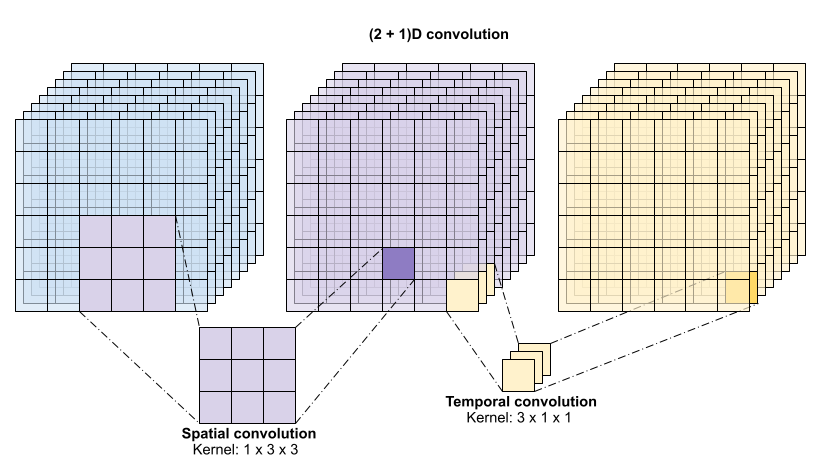
\includegraphics[width=0.70\textwidth]{../figuras/2plus1CNN-converted.png}
    \caption{Exemplo de decomposição de uma convolução espaço-temporal em convolução espacial e temporal. No contexto deste trabalho, a figura deve ser entendida apenas como ilustração complementar, pois mamografias convencionais são analisadas como imagens bidimensionais.}
    \label{fig:convolucao_2mais1d}
\end{figure}

Em mamografia, CNNs têm sido utilizadas em diversas tarefas, incluindo detecção e localização de lesões, classificação de exames, recuperação de imagens e avaliação de risco. Abdelhafiz et al. revisaram 83 estudos sobre CNNs aplicadas à mamografia e destacaram que técnicas como pré-processamento, uso de múltiplas vistas, transferência de aprendizado, aumento de dados, normalização em lote e \textit{dropout} são frequentemente empregadas para melhorar o desempenho e reduzir o sobreajuste \cite{abdelhafiz2019}.

Além disso, Abdelhafiz et al. indicam que a estrutura básica de uma CNN envolve a combinação de camadas convolucionais, funções não lineares, camadas de \textit{pooling} e uma etapa final de classificação, frequentemente baseada em \textit{softmax} \cite{abdelhafiz2019}. Essa estrutura permite que a rede receba uma imagem como entrada e produza como saída uma classe ou uma distribuição de probabilidades entre classes, como \textit{Normal}, \textit{Benign} e \textit{Malignant}.

Um exemplo de aplicação de CNN em mamografia é o estudo de Sundell et al. \cite{sundell2022cnn}, no qual diferentes arquiteturas convolucionais foram avaliadas para pontuação automática de imagens de controle de qualidade em mamografia. Os autores utilizaram blocos compostos por convolução, normalização, ativação ReLU, \textit{max pooling} e \textit{dropout}, demonstrando a aplicação prática desses componentes em uma tarefa relacionada à análise de imagens mamográficas.

Dessa forma, CNNs são especialmente adequadas para a classificação de mamografias porque combinam extração automática de características, preservação da estrutura espacial e capacidade de aprender representações hierárquicas. Ao mesmo tempo, seu uso exige atenção a desafios como alta resolução das imagens, desbalanceamento de classes, limitação de dados anotados, risco de sobreajuste, perda de detalhes durante operações de redução espacial e necessidade de interpretação clínica dos resultados.

\subsection{CNNs aplicadas à mamografia}

As redes neurais convolucionais tornaram-se uma das principais abordagens para análise computacional de imagens médicas, especialmente em tarefas de classificação, detecção e segmentação. Em mamografias, essas arquiteturas são utilizadas para extrair automaticamente padrões visuais associados a achados como massas, calcificações, assimetrias e distorções arquiteturais, reduzindo a dependência de técnicas manuais de extração de atributos.

A principal característica das CNNs é o uso de camadas convolucionais, que aplicam filtros sobre regiões locais da imagem para identificar padrões espaciais. Nas primeiras camadas, a rede tende a aprender características simples, como bordas, texturas e variações de intensidade. Nas camadas mais profundas, essas informações são combinadas em representações mais abstratas, capazes de auxiliar na distinção entre diferentes classes diagnósticas.

Em mamografias, o uso de CNNs apresenta desafios específicos. As imagens costumam ter alta resolução, baixo contraste em regiões de interesse e grande variabilidade entre pacientes, equipamentos e bases de dados. Além disso, lesões clinicamente relevantes podem ocupar pequenas regiões da imagem, o que exige modelos capazes de preservar informações espaciais importantes ao longo do processo de treinamento.

Por esse motivo, arquiteturas aplicadas à mamografia frequentemente combinam camadas convolucionais com técnicas de regularização, normalização, aumento de dados e estratégias de avaliação por classe. Essas escolhas são importantes para reduzir sobreajuste, melhorar a generalização e tornar o desempenho do modelo mais confiável em cenários com classes desbalanceadas.

\subsection{Explicabilidade e Grad-CAM}

A explicabilidade é um aspecto importante em modelos de aprendizado profundo aplicados a imagens médicas, pois decisões automatizadas em contextos clínicos precisam ser interpretáveis e avaliáveis por especialistas. Embora CNNs possam alcançar bom desempenho em tarefas de classificação, elas são frequentemente tratadas como modelos de difícil interpretação, uma vez que suas decisões resultam de múltiplas camadas de transformação não linear.

Uma das técnicas utilizadas para auxiliar a interpretação de CNNs é o Grad-CAM (\textit{Gradient-weighted Class Activation Mapping}). Essa abordagem gera mapas de calor que indicam quais regiões da imagem tiveram maior influência na decisão do modelo para determinada classe. Para isso, são utilizados os gradientes da saída de interesse em relação às ativações de uma camada convolucional profunda, produzindo uma visualização espacial das áreas mais relevantes para a predição.


%colocar imagem que eu gerei aqui?
Em mamografias, mapas Grad-CAM podem ajudar a verificar se o modelo está concentrando sua atenção em regiões anatomicamente plausíveis, como áreas de massa, assimetria ou calcificação. Entretanto, esses mapas não devem ser interpretados como laudos médicos nem como segmentações precisas de lesões. Seu papel é fornecer uma ferramenta complementar de interpretabilidade, permitindo identificar possíveis comportamentos indesejados do modelo, como foco em bordas, artefatos ou regiões externas à mama.

\section{Preparação, treinamento e avaliação de modelos supervisionados}

O desempenho de um modelo supervisionado não depende apenas da etapa de treinamento. Em problemas de imagens médicas, a preparação dos dados, a separação correta entre treino, validação e teste, o controle do desbalanceamento, a regularização e a escolha das métricas influenciam diretamente a confiabilidade dos resultados. Um modelo pode apresentar bons resultados aparentes quando treinado, mas ainda assim falhar em generalizar caso exista vazamento de dados, distribuição inadequada entre classes ou avaliação baseada apenas em acurácia global.

Por esse motivo, esta seção reúne os principais cuidados metodológicos necessários para que a comparação entre CNN clássica, CNN com gargalo clássico e modelo híbrido quântico-clássico seja conduzida de forma controlada. O objetivo não é apenas treinar redes, mas garantir que os resultados obtidos possam ser interpretados de maneira justa, reprodutível e coerente com a natureza sensível da classificação de mamografias.

\subsection{Qualidade dos rótulos, desbalanceamento e viés dos dados}
\label{subsec:qualidade_rotulos_balanceamento_vies}

Em tarefas de classificação supervisionada, o desbalanceamento de classes representa um problema metodológico relevante, pois modelos treinados com distribuições muito assimétricas tendem a favorecer a classe majoritária, reduzindo a capacidade de reconhecimento das classes menos representadas. Em aplicações médicas, esse problema é ainda mais sensível, uma vez que erros em classes minoritárias podem afetar diretamente a interpretação dos resultados e a utilidade clínica do modelo.

Segundo \cite{silva2025balanceamento}, técnicas de tratamento de dados desbalanceados podem ser organizadas em duas frentes principais: técnicas em nível de dados, como \textit{oversampling} e \textit{undersampling}, e técnicas em nível de algoritmo, como o \textit{cost-sensitive learning}, baseado em ajustes na função de perda ou na ponderação das classes. No entanto, a escolha da técnica deve ser documentada com cautela, pois o balanceamento altera a distribuição original dos dados e pode produzir impactos sobre o comportamento do modelo. Dessa forma, neste trabalho, o balanceamento das classes é adotado como uma etapa metodológica controlada, com o objetivo de reduzir o viés em direção à classe majoritária e permitir uma comparação mais justa entre os modelos avaliados.

\subsection{Preparação e tratamento dos dados}

A preparação dos dados envolve a definição dos subconjuntos experimentais, o controle de vazamento de dados, o tratamento do desbalanceamento, o aumento de dados e as estratégias de regularização necessárias para reduzir sobreajuste. Essas etapas são fundamentais para que a comparação entre os modelos seja conduzida sob condições controladas.

\subsection{Tratamento do desbalanceamento de classes}
\label{subsec:tratamento_desbalanceamento_classes}

O balanceamento de classes é um ponto metodológico central em tarefas de classificação de imagens médicas. Em bases de mamografia, é comum que a quantidade de exames normais seja maior do que a quantidade de exames benignos ou malignos. Quando essa distribuição é muito desigual, o modelo pode aprender a favorecer a classe majoritária, obtendo acurácia global aparentemente alta, mas baixo desempenho justamente nas classes clinicamente mais importantes. Por isso, a avaliação por métricas macro e por matriz de confusão deve ser acompanhada de uma estratégia explícita de tratamento do desbalanceamento.

De forma geral, uma base pode ser representada por classes \(C_0, C_1, \ldots, C_{K-1}\), cada uma com \(n_k\) amostras. O desbalanceamento ocorre quando:

\[
n_i \gg n_j
\quad \text{para algumas classes } i \text{ e } j.
\]

Nesse cenário, a função de perda média pode ser dominada pelas classes com mais exemplos, pois elas aparecem mais vezes durante o treinamento. Em mamografias, esse efeito é problemático porque uma classe menos frequente, como a classe maligna, pode ter maior relevância clínica do que a classe majoritária. Assim, o objetivo do balanceamento não é alterar artificialmente a distribuição real do problema, mas tornar o processo de aprendizagem menos enviesado durante o treinamento.

Silva \cite{silva2025balanceamento} discute técnicas de equilíbrio de classes e destaca que métodos de balanceamento podem modificar a distribuição dos dados, influenciando tanto o desempenho dos modelos quanto aspectos de privacidade. Embora o contexto da autora envolva ataques de inferência de associação, o balanceamento deve ser tratado como uma decisão metodológica explícita, e não como uma etapa automática sem impacto experimental.

Uma das técnicas mais conhecidas é o \textit{oversampling}, que aumenta a presença da classe minoritária no treinamento. Isso pode ser feito por repetição controlada de amostras ou por aumento de dados em imagens, desde que as transformações preservem características diagnósticas relevantes. Neste TCC, a sobreamostragem será tratada nesse sentido prático, como uma estratégia para expor o modelo mais vezes às classes menos representadas, sem introduzir técnicas sintéticas que não serão avaliadas no escopo do trabalho.

Além das técnicas em nível de dados, existe o \textit{cost-sensitive learning}, ou aprendizado sensível a custos. Nessa abordagem, a distribuição dos dados não é modificada diretamente. Em vez disso, a função de perda passa a atribuir pesos maiores aos erros cometidos nas classes mais relevantes ou menos representadas. De forma simplificada, uma perda ponderada pode ser escrita como:

\[
\mathcal{L}_{custo} =
\frac{1}{N}
\sum_{i=1}^{N}
w_{y_i}\mathcal{L}(y_i, f_{\theta}(x_i)),
\]

em que \(w_{y_i}\) representa o peso associado à classe verdadeira da amostra \(x_i\). Em uma tarefa de mamografia, essa estratégia pode ser útil porque erros envolvendo a classe maligna podem receber maior penalização do que erros em classes de menor criticidade clínica. Neste TCC, o \textit{cost-sensitive learning} não será assumido como técnica principal desde o início, mas poderá ser avaliado como alternativa ou experimento complementar, principalmente caso o balanceamento por reamostragem produza sobreajuste, descarte excessivo de amostras ou instabilidade nos resultados.

A Figura~\ref{fig:balanceamento_over_under_silva2025} mostra, de forma esquemática, duas estratégias clássicas: o \textit{oversampling}, que aumenta a quantidade de exemplos da classe minoritária, e o \textit{undersampling}, que reduz a quantidade de exemplos da classe majoritária. O oversampling tende a preservar todas as amostras disponíveis, mas pode aumentar o risco de sobreajuste se houver simples repetição excessiva. O undersampling reduz o custo de treinamento e diminui o domínio da classe majoritária, mas pode descartar exemplos úteis, especialmente quando a base já possui quantidade limitada de dados.

\begin{figure}[H]
    \centering
    \begin{minipage}{0.48\textwidth}
        \centering
        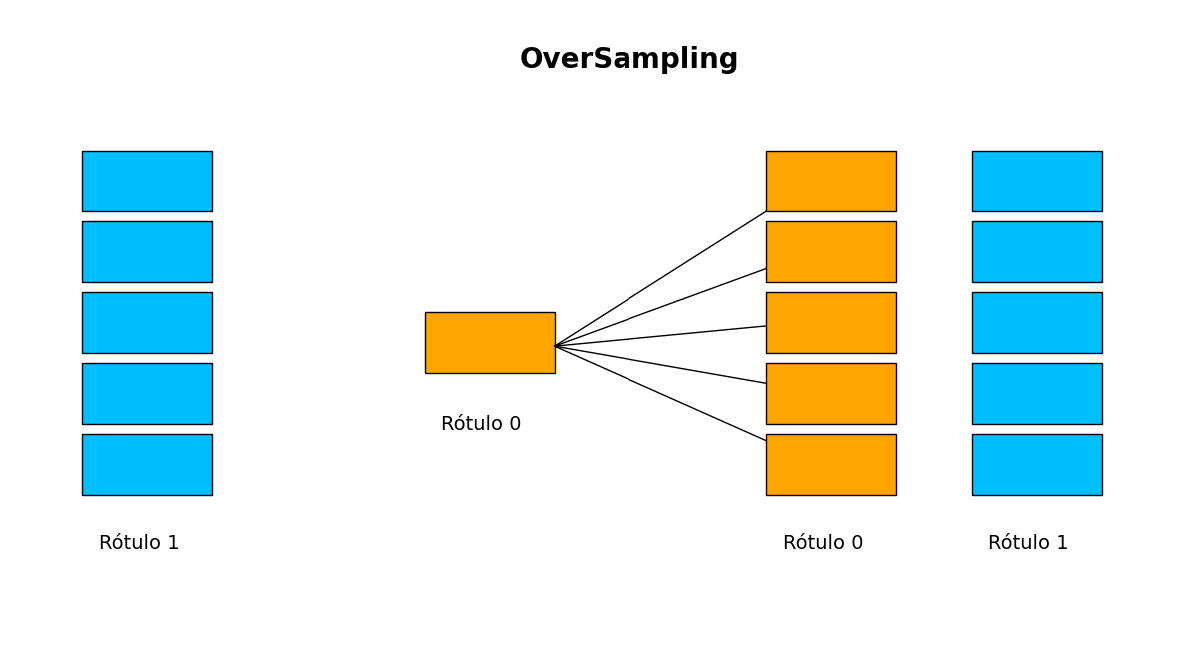
\includegraphics[width=\textwidth]{../figuras/balanceamento_oversampling_silva2025.png}
    \end{minipage}
    \hfill
    \begin{minipage}{0.48\textwidth}
        \centering
        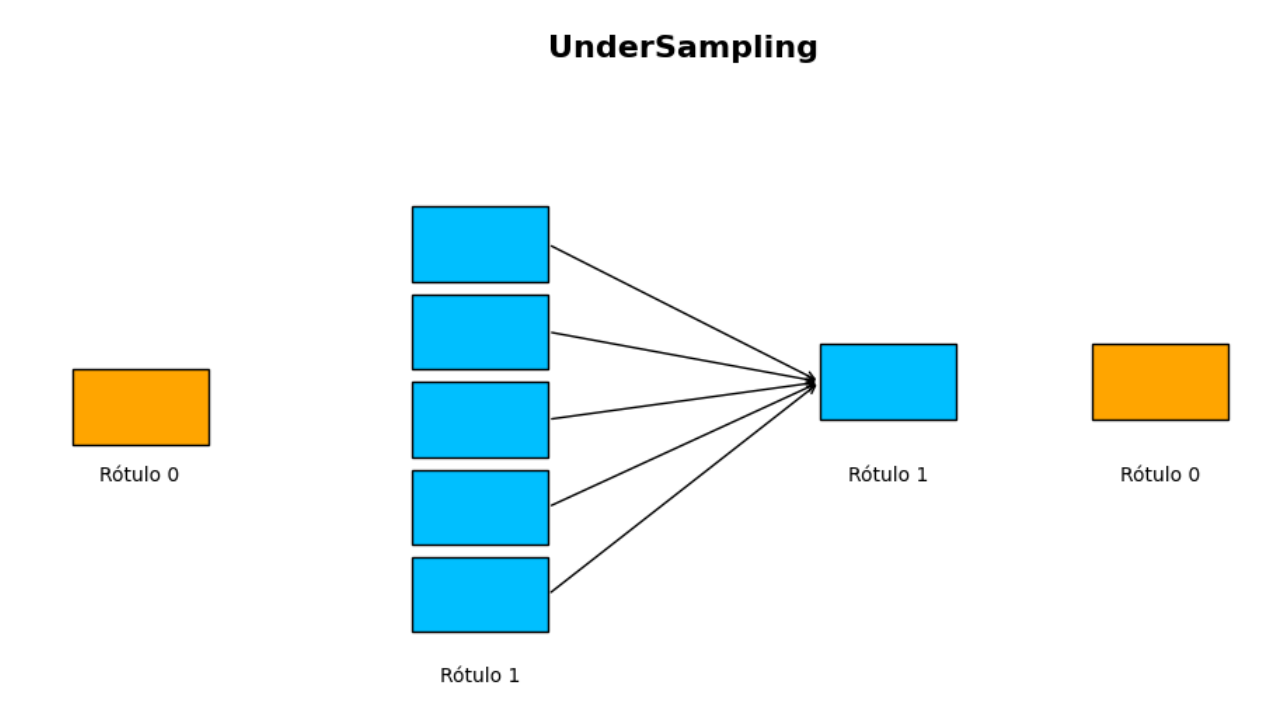
\includegraphics[width=\textwidth]{../figuras/balanceamento_undersampling_silva2025.png}
    \end{minipage}
    \caption{Representação visual de \textit{oversampling} e \textit{undersampling}.}
    \legend{Fonte: adaptado de \citeonline{silva2025balanceamento}.}
    \label{fig:balanceamento_over_under_silva2025}
\end{figure}

Neste trabalho será adotada uma estratégia híbrida de balanceamento, combinando \textit{oversampling} das classes minoritárias e \textit{undersampling} controlado da classe majoritária. A combinação é necessária porque o uso isolado de oversampling pode aumentar demais o número de exemplos repetidos ou aumentados, enquanto o uso isolado de undersampling pode remover informação relevante da classe mais frequente. A estratégia híbrida busca um ponto intermediário: reduzir o domínio da classe majoritária e, ao mesmo tempo, aumentar a exposição do modelo às classes menos representadas.

Esse balanceamento será aplicado apenas ao conjunto de treinamento. Os conjuntos de validação e teste deverão manter a distribuição original dos dados, pois eles representam a condição real de avaliação do modelo. Dessa forma, o balanceamento atua como estratégia de aprendizagem, mas não mascara o desempenho final. A validação será utilizada para seleção de hiperparâmetros e comparação intermediária entre configurações, enquanto o teste será reservado para a avaliação final. Caso seja útil para análise diagnóstica do comportamento dos modelos, poderá ser apresentado um relatório complementar com métricas por classe ou subconjuntos estratificados, mas o resultado principal deverá ser calculado sobre a distribuição original de teste. Os resultados serão avaliados com métricas sensíveis ao desbalanceamento, como F1-score macro, AUC macro, acurácia balanceada, recall da classe maligna e matriz de confusão por classe.

\subsection{Divisão entre treino, validação e teste}
\label{subsec:divisao_treino_validacao_teste}

Em aprendizado supervisionado, a avaliação adequada de um modelo depende da separação do conjunto de dados em subconjuntos com funções distintas. De modo geral, os dados são divididos em treino, validação e teste. O conjunto de treino é utilizado para ajustar os parâmetros do modelo; o conjunto de validação auxilia no acompanhamento do desempenho e na escolha de hiperparâmetros; e o conjunto de teste é reservado para estimar o desempenho final em dados não vistos.

Essa divisão é essencial porque o objetivo de um modelo de aprendizado de máquina não é apenas memorizar os exemplos usados no treinamento, mas generalizar para novas amostras. Deisenroth, Faisal e Ong ressaltam que o aprendizado deve buscar desempenho em dados ainda não observados, e não apenas bom ajuste aos dados disponíveis \cite{deisenroth2020mathematics}. Em imagens médicas, essa questão é especialmente importante, pois um modelo pode obter bons resultados em uma base específica e ainda assim apresentar desempenho inferior quando aplicado a imagens de outra instituição, equipamento ou população.

\subsection{Treinamento, função de perda e generalização}
\label{subsec:treinamento_funcao_perda_generalizacao}

Durante o treinamento, o modelo recebe os exemplos do conjunto de treino e atualiza seus parâmetros com base no erro calculado. Considerando uma função de perda \(\mathcal{L}\), o treinamento pode ser descrito pela minimização do risco empírico:

\[
R_{\text{emp}}(\theta)
=
\frac{1}{N}
\sum_{i=1}^{N}
\mathcal{L}(y_i, f_{\theta}(x_i)).
\]

O risco empírico mede o erro médio do modelo sobre os dados disponíveis para treinamento. No entanto, o interesse real está no desempenho esperado em dados novos. A diferença entre o erro de treino e o erro em validação ou teste está relacionada à capacidade de generalização do modelo.

A atualização dos parâmetros pode ser representada, de forma simplificada, por uma etapa de gradiente descendente:

\[
\theta_{t+1}
=
\theta_t
-
\eta
\nabla_{\theta}
R_{\text{emp}}(\theta_t),
\]

em que \(\theta_t\) representa os parâmetros na iteração \(t\), \(\eta\) é a taxa de aprendizado e \(\nabla_{\theta}R_{\text{emp}}(\theta_t)\) é o gradiente da função de perda em relação aos parâmetros. Esse processo é repetido ao longo de várias épocas, até que o modelo alcance um desempenho adequado ou até que critérios de parada sejam satisfeitos.

O conjunto de validação é utilizado para acompanhar o comportamento do modelo durante o treinamento. Ele permite verificar se a redução da perda no treino está acompanhada de melhora em dados não utilizados diretamente na atualização dos pesos. Além disso, a validação auxilia na escolha de hiperparâmetros, como taxa de aprendizado, tamanho do lote, número de épocas, profundidade da rede, intensidade de regularização e estratégia de aumento de dados.

O conjunto de teste, por sua vez, deve ser utilizado somente ao final do processo de desenvolvimento. Sua função é fornecer uma estimativa mais imparcial do desempenho final do modelo. Caso o conjunto de teste seja usado repetidamente para tomar decisões de modelagem, ele deixa de representar uma avaliação independente, pois passa a influenciar indiretamente o ajuste do modelo.

A generalização pode ser compreendida como a capacidade do modelo de manter desempenho satisfatório em exemplos que não participaram do treinamento. Quando o modelo apresenta baixo erro no treino, mas erro elevado na validação ou no teste, ocorre o fenômeno conhecido como \textit{overfitting}, ou sobreajuste. Nesse caso, o modelo aprende detalhes específicos do conjunto de treino, como ruídos, artefatos, padrões de aquisição ou características particulares da base, em vez de aprender padrões gerais associados às classes.

O comportamento típico do sobreajuste pode ser representado por:

\[
\mathcal{L}_{train} \downarrow
\quad \text{e} \quad
\mathcal{L}_{val} \uparrow,
\]

ou seja, a perda de treino continua diminuindo enquanto a perda de validação aumenta ou deixa de melhorar. Também pode ocorrer quando a acurácia de treino cresce continuamente, mas a acurácia de validação se estabiliza ou diminui. Goodfellow, Bengio e Courville discutem esse problema como uma das principais limitações de modelos de alta capacidade, especialmente quando a quantidade de dados é limitada em relação ao número de parâmetros treináveis \cite{goodfellow2016deep}.

O fenômeno oposto é o \textit{underfitting}, ou subajuste. Ele ocorre quando o modelo não consegue aprender adequadamente nem mesmo os padrões presentes no conjunto de treino. Nesse caso, tanto o desempenho no treino quanto o desempenho na validação permanecem baixos. O subajuste pode ocorrer quando o modelo é simples demais, quando o treinamento é insuficiente ou quando as características extraídas não são adequadas para a tarefa.

Em mamografias, a generalização é um desafio particular. Abdelhafiz et al. indicam que o treinamento de redes profundas em mamografia é dificultado pela disponibilidade limitada de dados médicos anotados, pela presença de bases com diferentes formatos e resoluções, pela necessidade de pré-processamento e pela possibilidade de desbalanceamento entre classes \cite{abdelhafiz2019}. Os autores também destacam que práticas como aumento de dados, transferência de aprendizado, normalização, \textit{dropout} e escolha adequada da validação são usadas para reduzir sobreajuste e melhorar a capacidade de generalização dos modelos.

Outro ponto importante é a definição da estratégia de validação. Em aprendizado profundo aplicado à mamografia, podem ser utilizadas estratégias como divisão simples em treino e teste, divisão em treino, validação e teste, ou validação cruzada \(k\)-fold. Abdelhafiz et al. descrevem que a validação cruzada é uma técnica estatística utilizada para avaliar modelos preditivos por meio da partição dos dados em subconjuntos, sendo comum em estudos com bases menores de mamografia \cite{abdelhafiz2019}. Em bases maiores, a separação em treino, validação e teste costuma ser uma alternativa prática, desde que realizada de forma estratificada e sem vazamento de dados.

O vazamento de dados, ou \textit{data leakage}, ocorre quando informações do conjunto de validação ou teste aparecem direta ou indiretamente no treinamento. Em imagens médicas, isso pode ocorrer, por exemplo, se imagens da mesma paciente, do mesmo exame ou de exames muito semelhantes forem distribuídas entre subconjuntos diferentes. Nessa situação, o modelo pode apresentar desempenho artificialmente elevado, pois aprende características específicas da paciente ou do exame, e não padrões gerais da doença.

Além disso, em bases desbalanceadas, a divisão dos dados deve preservar a distribuição das classes entre treino, validação e teste. Essa estratégia é conhecida como divisão estratificada. Caso uma classe fique sub-representada em algum subconjunto, a avaliação pode se tornar instável ou pouco representativa. Em mamografias, esse cuidado é relevante porque classes malignas tendem a ser menos frequentes do que exames normais em bases de rastreamento.

O estudo de Sundell et al. ilustra a importância da separação entre dados de treinamento, validação e teste em aplicações de CNNs na mamografia. Os autores utilizaram imagens de controle de qualidade mamográfica para treinar modelos supervisionados, separando dados de treino/validação e avaliando o desempenho em um conjunto de teste independente, composto por imagens de diferentes condições de qualidade e dose \cite{sundell2022cnn}. Além disso, o trabalho evidencia que o aumento da complexidade da rede pode melhorar o desempenho até certo ponto, mas também pode prejudicar a generalização quando há excesso de camadas ou parâmetros.

Portanto, treinamento, validação, teste e generalização são conceitos centrais para a construção de modelos confiáveis em classificação de imagens médicas. O treino ajusta os parâmetros do modelo; a validação orienta decisões de configuração e controle de sobreajuste; e o teste estima o desempenho final em dados não utilizados no desenvolvimento. Em mamografias, essa separação deve ser conduzida com cuidado devido à alta dimensionalidade das imagens, à presença de padrões sutis, ao desbalanceamento das classes, à variabilidade entre bases e ao risco de vazamento de dados.

\subsection{Overfitting, underfitting e regularização}
\label{subsec:aumento_regularizacao_overfitting}

O treinamento de redes neurais profundas exige cuidado com a capacidade de generalização do modelo. Em aprendizado supervisionado, o objetivo não é apenas reduzir o erro sobre os dados de treinamento, mas obter bom desempenho em exemplos ainda não vistos. Esse princípio é especialmente importante em imagens médicas, pois modelos de alta capacidade podem aprender padrões específicos da base utilizada, como ruídos, artefatos de aquisição, bordas, marcas ou características do equipamento, em vez de aprender padrões clinicamente relevantes.

Em termos matemáticos, considera-se um conjunto de treinamento:

\[
\mathcal{D}_{train} = \{(x_1,y_1),(x_2,y_2),\ldots,(x_N,y_N)\},
\]

em que \(x_i\) representa uma imagem e \(y_i\) seu respectivo rótulo. O treinamento busca ajustar os parâmetros \(\theta\) de um modelo \(f_{\theta}\) minimizando uma função de perda média, também chamada de risco empírico:

\[
R_{\text{emp}}(\theta) =
\frac{1}{N}
\sum_{i=1}^{N}
\mathcal{L}(y_i, f_{\theta}(x_i)).
\]

Entretanto, minimizar excessivamente essa perda no conjunto de treino não garante bom desempenho em dados novos. Quando o modelo apresenta baixo erro no treino, mas erro elevado na validação ou no teste, ocorre o fenômeno conhecido como \textit{overfitting}, ou sobreajuste. Nesse caso, a rede aprende detalhes específicos dos exemplos de treinamento, reduzindo sua capacidade de generalização. Por outro lado, quando o modelo é simples demais ou treinado de forma insuficiente, pode ocorrer \textit{underfitting}, situação em que o desempenho é baixo tanto no treino quanto na validação.

Uma forma de reduzir o sobreajuste é aplicar regularização. A regularização introduz restrições ou penalizações ao processo de aprendizagem, buscando impedir que o modelo se ajuste de forma excessiva aos dados de treino. Uma formulação comum consiste em adicionar um termo de penalização à função objetivo:

\[
J(\theta) =
\frac{1}{N}
\sum_{i=1}^{N}
\mathcal{L}(y_i, f_{\theta}(x_i))
+
\lambda \Omega(\theta),
\]

em que \(\Omega(\theta)\) é o termo de regularização e \(\lambda\) controla a intensidade da penalização. Quando se utiliza regularização \(L_2\), por exemplo, a penalização pode ser definida como:

\[
\Omega(\theta) = \|\theta\|_2^2.
\]

Nesse caso, pesos muito altos são penalizados, incentivando o modelo a encontrar soluções mais suaves e menos dependentes de parâmetros extremos. Essa estratégia pode melhorar a generalização, pois reduz a tendência da rede de memorizar detalhes específicos dos dados de treino \cite{goodfellow2016deep}.

Outra técnica amplamente utilizada é o \textit{dropout}. Durante o treinamento, o dropout desativa aleatoriamente uma proporção dos neurônios de uma camada, forçando a rede a distribuir melhor a informação entre diferentes unidades. Se \(h\) representa o vetor de ativações de uma camada, o dropout pode ser representado de forma simplificada como:

\[
\tilde{h} = m \odot h,
\]

em que \(m\) é uma máscara binária aleatória, \(\odot\) representa o produto elemento a elemento e \(\tilde{h}\) corresponde às ativações após a aplicação da máscara. Essa técnica reduz a dependência excessiva de neurônios específicos e contribui para tornar o modelo mais robusto.

Outra técnica relacionada à regularização é o \textit{early stopping}. Nesse procedimento, o desempenho do modelo é monitorado no conjunto de validação durante o treinamento. Quando a perda de validação deixa de melhorar por um número definido de épocas, o treinamento é interrompido. Essa estratégia evita que o modelo continue reduzindo a perda de treino enquanto piora sua capacidade de generalização. Em termos práticos, o comportamento típico de sobreajuste pode ser observado quando:

\[
\mathcal{L}_{train} \downarrow
\quad \text{e} \quad
\mathcal{L}_{val} \uparrow
\]

ou quando a acurácia de treino continua aumentando enquanto a acurácia de validação se estabiliza ou diminui.

\subsection{Aumento de dados em imagens médicas}
\label{subsec:aumento_dados_imagens_medicas}

Além da regularização dos parâmetros, outra estratégia importante é o aumento de dados, ou \textit{data augmentation}. Essa técnica consiste em gerar variações artificiais das imagens de treinamento por meio de transformações que preservam o rótulo da amostra. Matematicamente, uma imagem \(x_i\) pode ser transformada por uma função \(T\), produzindo uma nova amostra:

\[
x_i' = T(x_i),
\]

em que \(x_i'\) mantém o mesmo rótulo \(y_i\), desde que a transformação não altere o significado clínico da imagem. Em imagens naturais, são comuns transformações como rotações, translações, espelhamentos, variações de brilho, contraste e recortes. Em mamografias, essas transformações devem ser escolhidas com cuidado, pois alterações inadequadas podem modificar estruturas relevantes ou gerar imagens incompatíveis com a prática clínica.

No contexto da mamografia, o aumento de dados pode incluir pequenas variações geométricas, ajustes leves de brilho e contraste, ruído controlado e técnicas de recorte ou mascaramento, desde que preservem características diagnósticas importantes. Essas transformações aumentam a diversidade observada pelo modelo durante o treinamento e reduzem a probabilidade de memorização de imagens específicas. Revisões sobre CNNs aplicadas à mamografia destacam que estratégias como pré-processamento, aumento de dados, normalização, dropout e ajuste cuidadoso da arquitetura são frequentemente utilizadas para melhorar desempenho e reduzir sobreajuste \cite{abdelhafiz2019}.

\begin{figure}[H]
    \centering
    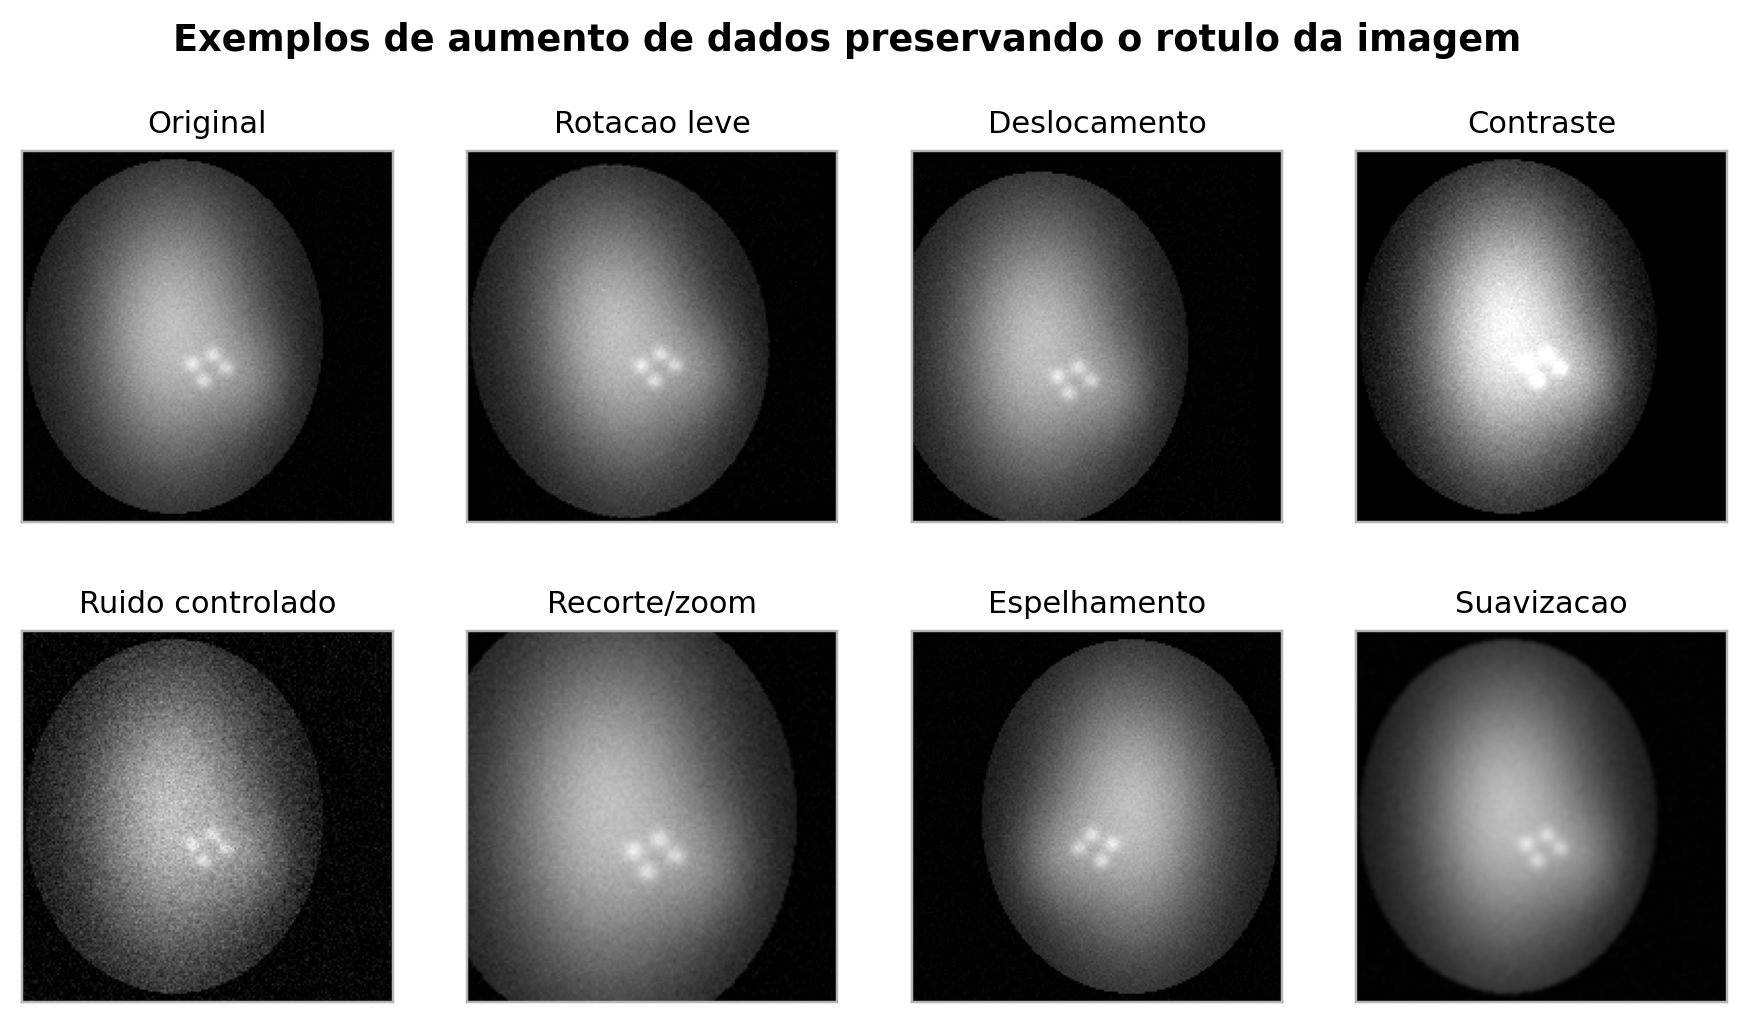
\includegraphics[width=\textwidth]{../figuras/aumento_dados_exemplos.png}
    \caption{Exemplos de aumento de dados por transformações leves aplicadas a uma imagem sintética em escala de cinza. As transformações ilustram alterações controladas que podem ampliar a diversidade do conjunto de treinamento sem modificar o rótulo da amostra. Fonte: elaborado pelo autor.}
    \label{fig:aumento_dados_exemplos}
\end{figure}

Em imagens médicas, o controle do sobreajuste é ainda mais importante devido a fatores como quantidade limitada de dados anotados, desbalanceamento entre classes, alta dimensionalidade das imagens e diferenças entre bases de origem. Em mamografias, pequenas regiões podem conter informações clinicamente relevantes, mas também é possível que o modelo aprenda padrões indesejados, como diferenças de contraste, ruído, marcas laterais ou características específicas de determinado equipamento. Por isso, a avaliação deve considerar não apenas o desempenho no treino, mas também métricas em validação e teste, preferencialmente analisadas por classe.

Portanto, aumento de dados, regularização, dropout, normalização e early stopping são estratégias complementares para melhorar a generalização de redes neurais profundas. No caso da classificação de mamografias, essas técnicas são fundamentais para reduzir o risco de sobreajuste e tornar a comparação entre modelos mais confiável, especialmente quando se trabalha com bases compostas por diferentes fontes, tamanhos de imagem, distribuições de classe e padrões de aquisição.

\subsection{Métricas de avaliação em classificação de mamografias}
\label{subsec:metricas_avaliacao}

A avaliação de modelos de classificação em imagens médicas deve ser compreendida a partir da formulação matemática geral do aprendizado supervisionado. Nesse contexto, considera-se um conjunto de dados composto por pares de entrada e rótulo:

\[
\mathcal{D} = \{(x_1,y_1),(x_2,y_2),\ldots,(x_N,y_N)\},
\]

em que \(x_i\) representa uma imagem de entrada e \(y_i\) representa seu rótulo verdadeiro. No caso da classificação de mamografias, \(x_i\) pode corresponder a uma imagem mamográfica representada numericamente, enquanto \(y_i\) pertence ao conjunto de classes diagnósticas possíveis, como \textit{Normal}, \textit{Benign} e \textit{Malignant}.

Segundo Deisenroth, Faisal e Ong, a aprendizagem de máquina pode ser entendida a partir de três componentes principais: dados, modelo e aprendizagem. Os dados são representados numericamente, frequentemente como vetores ou matrizes; o modelo é uma função parametrizada; e a aprendizagem consiste em ajustar os parâmetros desse modelo a partir dos dados disponíveis, buscando bom desempenho em dados não vistos \cite{deisenroth2020mathematics}. Assim, em uma tarefa de classificação, o modelo pode ser representado por uma função parametrizada:

\[
f_{\theta}: \mathbb{R}^{D} \rightarrow \mathbb{R}^{K},
\]

em que \(D\) representa a dimensão da entrada após sua representação numérica, \(K\) representa o número de classes e \(\theta\) representa o conjunto de parâmetros do modelo.

Em redes neurais aplicadas à classificação multiclasse, a saída do modelo geralmente é transformada em um vetor de probabilidades por meio da função \textit{softmax}. Para uma imagem \(x_i\), o modelo produz um vetor:

\[
\hat{p}_i = f_{\theta}(x_i) = [p_{i,0}, p_{i,1}, \ldots, p_{i,K-1}],
\]

em que \(p_{i,k}\) representa a probabilidade estimada de a imagem \(x_i\) pertencer à classe \(k\). A classe prevista pelo modelo é obtida por:

\[
\hat{y}_i = \arg\max_{k} p_{i,k}.
\]

Durante o treinamento, o objetivo é minimizar uma função de perda, isto é, uma medida matemática do erro entre a predição do modelo e o rótulo verdadeiro. A formulação de minimização do risco empírico expressa esse processo como a minimização da média das perdas no conjunto de treinamento:

\[
R_{\text{emp}}(f_{\theta}) =
\frac{1}{N}
\sum_{i=1}^{N}
\ell(y_i, f_{\theta}(x_i)),
\]

em que \(\ell\) representa a função de perda. Para classificação multiclasse, uma função frequentemente utilizada é a entropia cruzada categórica, definida por:

\[
\mathcal{L}(y_i, \hat{p}_i) =
-\sum_{k=0}^{K-1} y_{i,k}\log(p_{i,k}),
\]

em que \(y_{i,k}\) representa o rótulo verdadeiro em codificação \textit{one-hot}. Quando a classe correta é \(c\), essa expressão se reduz a:

\[
\mathcal{L}(y_i, \hat{p}_i) = -\log(p_{i,c}).
\]

Dessa forma, a perda será baixa quando o modelo atribuir alta probabilidade à classe correta e será alta quando o modelo atribuir baixa probabilidade à classe verdadeira. Entretanto, a função de perda utilizada no treinamento não é suficiente para avaliar completamente o desempenho do modelo em um problema médico. Por isso, além da perda, são utilizadas métricas de avaliação calculadas sobre o conjunto de validação ou teste.

A métrica mais direta é a acurácia, que mede a proporção de classificações corretas em relação ao total de amostras avaliadas:

\[
Accuracy =
\frac{1}{N}
\sum_{i=1}^{N}
\mathbb{1}(\hat{y}_i = y_i),
\]

em que \(\mathbb{1}(\hat{y}_i = y_i)\) é uma função indicadora que assume valor 1 quando a predição está correta e 0 caso contrário. Embora seja uma métrica intuitiva, a acurácia pode ser insuficiente em bases desbalanceadas. Por exemplo, se uma base possui muitas imagens normais e poucas imagens malignas, um modelo pode obter acurácia aparentemente alta apenas por favorecer a classe majoritária.

Para uma análise mais detalhada, utiliza-se a matriz de confusão. Em um problema com \(K\) classes, a matriz de confusão pode ser representada por:

\[
C \in \mathbb{N}^{K \times K},
\]

em que cada elemento \(C_{ij}\) indica a quantidade de exemplos cuja classe verdadeira é \(i\) e cuja classe prevista é \(j\). Para três classes, a matriz pode ser representada como:

\[
C =
\begin{bmatrix}
C_{00} & C_{01} & C_{02} \\
C_{10} & C_{11} & C_{12} \\
C_{20} & C_{21} & C_{22}
\end{bmatrix}.
\]

Os elementos da diagonal principal representam os acertos do modelo, enquanto os elementos fora da diagonal representam erros de classificação. Por exemplo, considerando as classes \textit{Normal}, \textit{Benign} e \textit{Malignant}, o elemento \(C_{02}\) representa imagens verdadeiramente normais classificadas como malignas, enquanto \(C_{20}\) representa imagens malignas classificadas incorretamente como normais.

A partir da matriz de confusão, é possível calcular métricas específicas por classe usando a estratégia \textit{one-vs-rest}. Nessa abordagem, para cada classe \(k\), considera-se essa classe como positiva e todas as demais como negativas. Assim, definem-se:

\[
TP_k = C_{kk},
\]

\[
FN_k =
\sum_{\substack{j=0 \\ j \neq k}}^{K-1}
C_{kj},
\]

\[
FP_k =
\sum_{\substack{i=0 \\ i \neq k}}^{K-1}
C_{ik},
\]

\[
TN_k =
\sum_{\substack{i=0 \\ i \neq k}}^{K-1}
\sum_{\substack{j=0 \\ j \neq k}}^{K-1}
C_{ij}.
\]

Nessas expressões, \(TP_k\) representa os verdadeiros positivos da classe \(k\), isto é, exemplos da classe \(k\) corretamente classificados como \(k\). \(FN_k\) representa os falsos negativos, ou seja, exemplos da classe \(k\) classificados como outra classe. \(FP_k\) representa os falsos positivos, isto é, exemplos de outras classes classificados incorretamente como \(k\). Por fim, \(TN_k\) representa os verdadeiros negativos, ou seja, exemplos que não pertencem à classe \(k\) e também não foram classificados como \(k\).

A precisão da classe \(k\) é definida por:

\[
Precision_k =
\frac{TP_k}{TP_k + FP_k}.
\]

Essa métrica indica, entre todas as imagens classificadas pelo modelo como pertencentes à classe \(k\), quantas realmente pertencem a essa classe. No contexto de mamografias, uma baixa precisão para a classe \textit{Malignant} indica que muitas imagens classificadas como malignas não eram, de fato, malignas, aumentando a ocorrência de falsos positivos.

A revocação, também chamada de sensibilidade em contextos médicos, é definida por:

\[
Recall_k = Sensitivity_k =
\frac{TP_k}{TP_k + FN_k}.
\]

Essa métrica indica a proporção de exemplos reais da classe \(k\) que foram corretamente identificados pelo modelo. Para a classe \textit{Malignant}, a revocação é especialmente importante, pois uma baixa revocação significa que muitos casos malignos foram classificados incorretamente como normais ou benignos, caracterizando falsos negativos.

A especificidade mede a capacidade do modelo de reconhecer corretamente os exemplos que não pertencem à classe analisada:

\[
Specificity_k =
\frac{TN_k}{TN_k + FP_k}.
\]

Enquanto a sensibilidade mede a capacidade de detectar corretamente os casos positivos, a especificidade mede a capacidade de evitar falsos alarmes. Em aplicações médicas, essas duas métricas devem ser analisadas em conjunto, pois um modelo pode ser muito sensível, mas pouco específico, ou o contrário.

O F1-score combina precisão e revocação por meio da média harmônica:

\[
F1_k =
2 \cdot
\frac{Precision_k \cdot Recall_k}
{Precision_k + Recall_k}.
\]

A média harmônica penaliza situações em que uma das duas métricas é baixa. Portanto, o F1-score só será elevado quando precisão e revocação forem simultaneamente altas. Essa característica torna o F1-score útil em problemas nos quais falsos positivos e falsos negativos são ambos relevantes.

Em problemas multiclasse, é comum calcular médias das métricas por classe. A média macro considera todas as classes com o mesmo peso:

\[
Macro\text{-}F1 =
\frac{1}{K}
\sum_{k=0}^{K-1}
F1_k.
\]

Já a média ponderada considera a quantidade de exemplos de cada classe:

\[
Weighted\text{-}F1 =
\sum_{k=0}^{K-1}
\frac{n_k}{N}
F1_k,
\]

em que \(n_k\) é o número de exemplos da classe \(k\) e \(N\) é o número total de exemplos. A média macro é importante quando se deseja avaliar se o modelo apresenta desempenho equilibrado entre as classes, enquanto a média ponderada reflete mais fortemente o desempenho nas classes com maior quantidade de amostras.

Outra métrica relevante em bases desbalanceadas é a acurácia balanceada, definida como a média das revocações por classe:

\[
Balanced\ Accuracy =
\frac{1}{K}
\sum_{k=0}^{K-1}
Recall_k.
\]

Essa métrica reduz o efeito da classe majoritária, pois cada classe contribui igualmente para o resultado final. Em mamografias, isso é importante porque classes clinicamente relevantes, como \textit{Benign} e \textit{Malignant}, podem ter menos amostras do que a classe \textit{Normal}.

Além dessas métricas, a curva ROC e a AUC são frequentemente utilizadas para avaliar a capacidade discriminativa do modelo. Para cada classe \(k\), considerando a estratégia \textit{one-vs-rest}, define-se a taxa de verdadeiros positivos como:

\[
TPR_k =
\frac{TP_k}{TP_k + FN_k},
\]

e a taxa de falsos positivos como:

\[
FPR_k =
\frac{FP_k}{FP_k + TN_k}.
\]

A curva ROC representa a relação entre \(TPR_k\) e \(FPR_k\) para diferentes limiares de decisão. A área sob essa curva, chamada AUC, pode ser expressa como:

\[
AUC_k =
\int_{0}^{1}
TPR_k(FPR_k)\,dFPR_k.
\]

Em termos práticos, a AUC mede a capacidade do modelo de atribuir pontuações mais altas aos exemplos positivos do que aos negativos. Valores próximos de \(0{,}5\) indicam desempenho semelhante ao acaso, enquanto valores próximos de \(1{,}0\) indicam alta capacidade de separação entre a classe analisada e as demais.

Portanto, a avaliação de modelos aplicados à classificação de mamografias não deve depender apenas da acurácia global. A matriz de confusão, a precisão, a revocação, a especificidade, o F1-score, a acurácia balanceada e a AUC fornecem uma análise mais completa do comportamento do modelo. Essa abordagem é coerente com a formulação matemática da aprendizagem de máquina, na qual o objetivo não é apenas minimizar o erro no conjunto de treinamento, mas estimar se o modelo é capaz de generalizar para dados não vistos \cite{deisenroth2020mathematics}. Em imagens médicas, essa análise é essencial porque diferentes tipos de erro possuem diferentes implicações clínicas.

\begin{figure}[H]
    \centering
    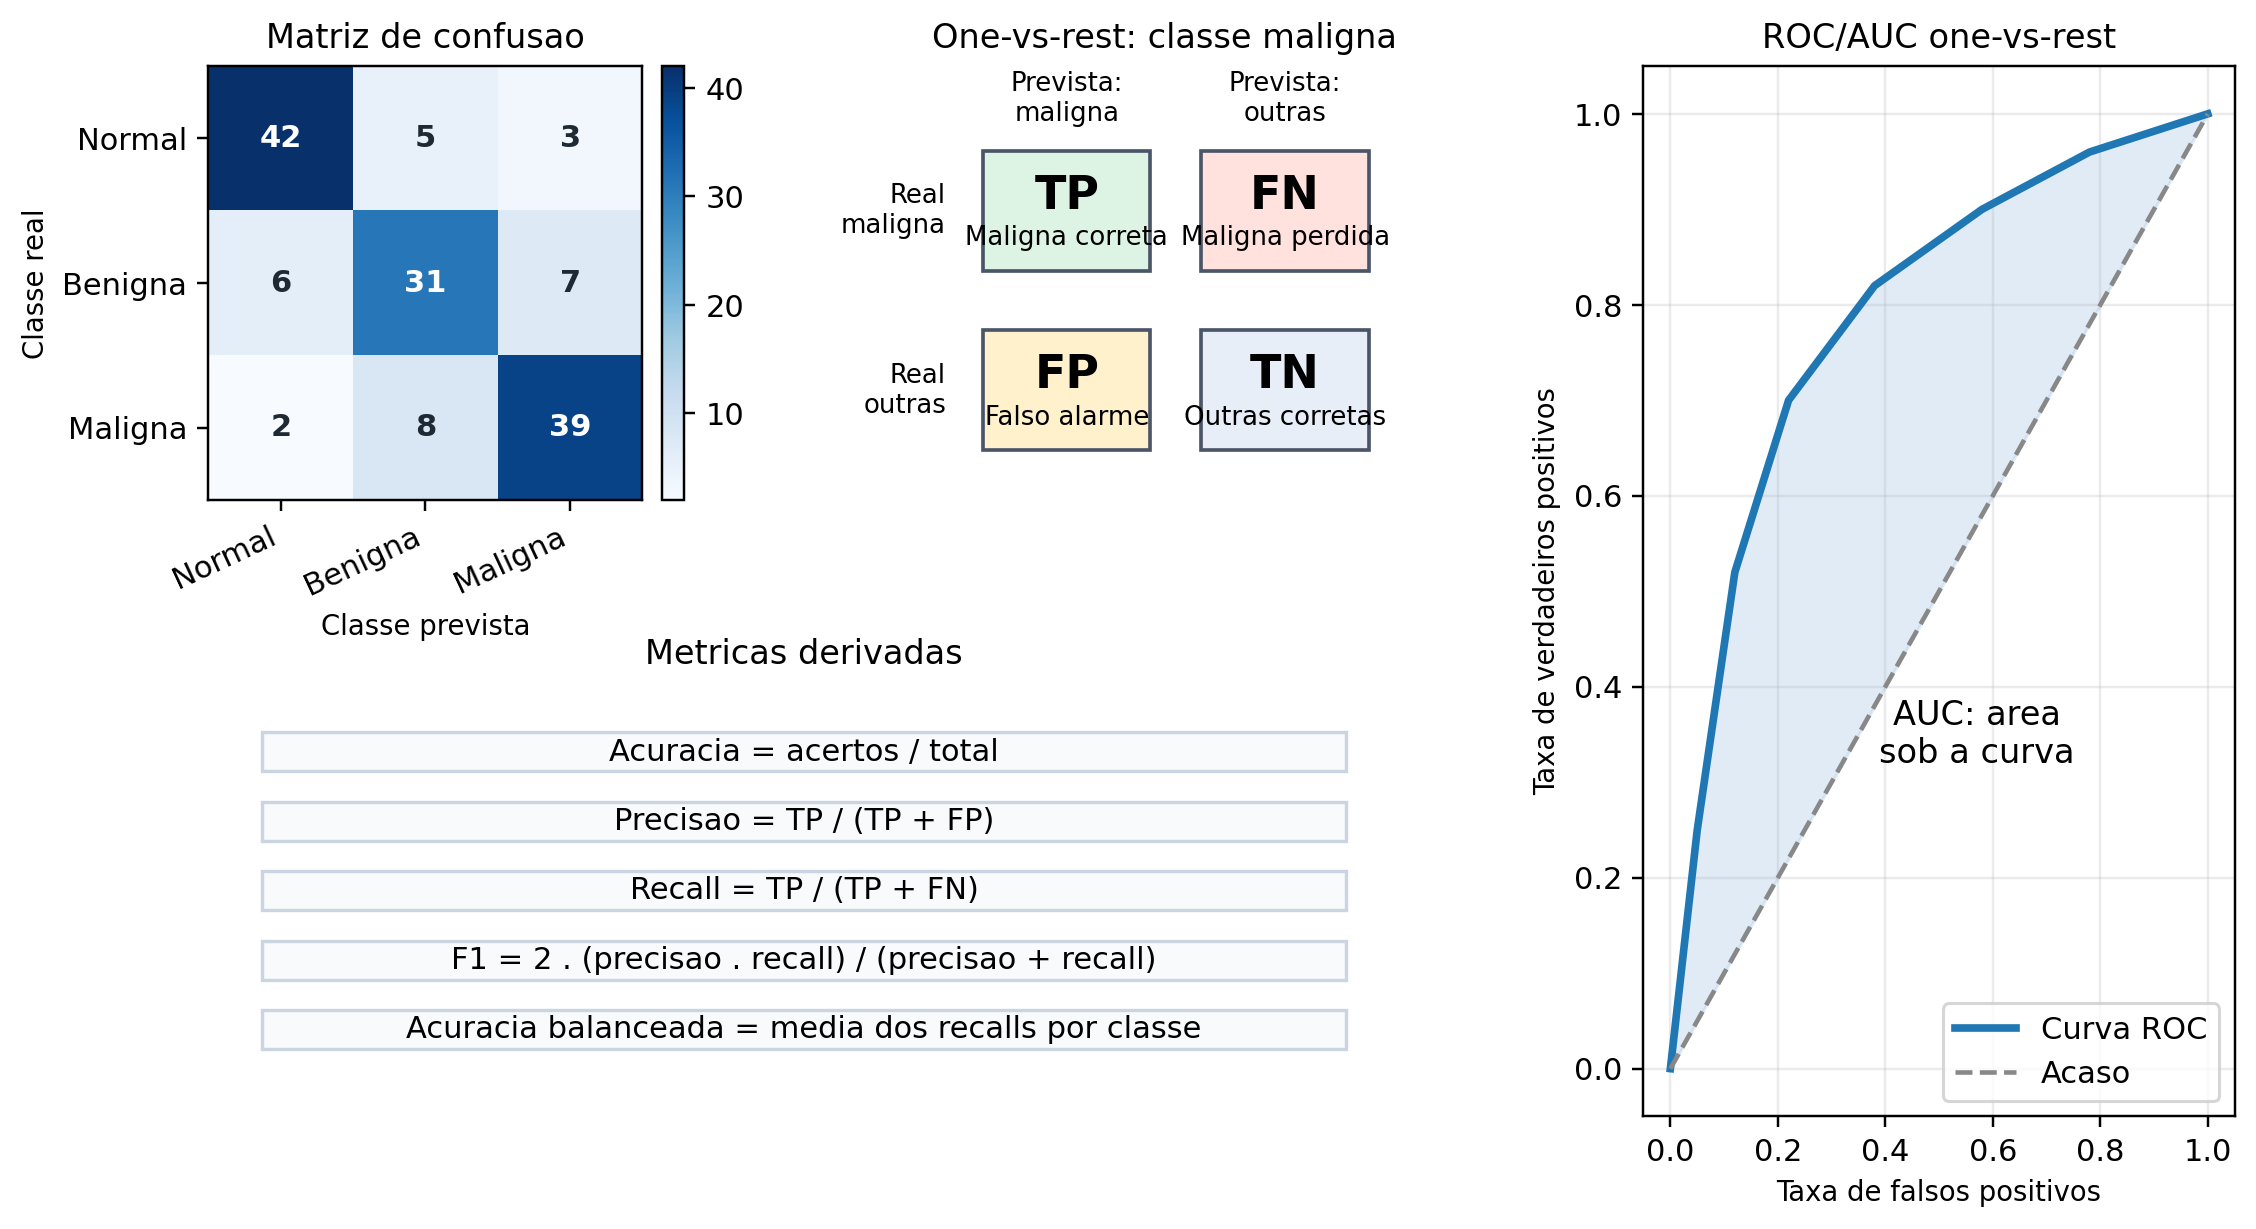
\includegraphics[width=\textwidth]{../figuras/metricas_classificacao_exemplos.png}
    \caption{Resumo visual de métricas utilizadas na avaliação de classificadores. A matriz de confusão permite identificar acertos e erros por classe; a estratégia \textit{one-vs-rest} organiza \(TP\), \(FP\), \(FN\) e \(TN\); e a curva ROC/AUC sintetiza a capacidade discriminativa do modelo em diferentes limiares. Fonte: elaborado pelo autor.}
    \label{fig:metricas_classificacao_exemplos}
\end{figure}

\subsection{Métricas de custo computacional e estabilidade experimental}
\label{subsec:metricas_custo_estabilidade}

Além das métricas preditivas, a comparação entre uma CNN clássica, uma CNN com gargalo clássico e um modelo híbrido quântico-clássico deve considerar custo computacional e estabilidade experimental. Para isso, podem ser acompanhados o tempo de treinamento, o tempo médio de inferência, o consumo de memória, o número de parâmetros treináveis, o número de épocas até a convergência e, no caso do modelo híbrido, o número de qubits, a profundidade do circuito, o número de \textit{shots} e o tempo de simulação.

A estabilidade experimental também deve ser analisada porque modelos de aprendizado profundo e circuitos variacionais podem apresentar variação entre execuções. Assim, sempre que viável, os experimentos devem registrar sementes aleatórias, médias, desvios-padrão e comportamento da curva de treinamento. Essa análise evita que a comparação dependa apenas de uma execução isolada e permite avaliar se eventuais diferenças de desempenho são consistentes.

\subsection{Comparação controlada entre modelos}
\label{subsec:comparacao_controlada_modelos}

A comparação entre os modelos deve ser conduzida sob o mesmo protocolo experimental. Isso significa utilizar a mesma base de dados, as mesmas classes, a mesma divisão entre treino, validação e teste, o mesmo pré-processamento, as mesmas métricas e critérios equivalentes de parada e seleção de hiperparâmetros. Dessa forma, a diferença observada entre os modelos pode ser interpretada com menor risco de ser causada por mudanças externas ao método avaliado.

Neste trabalho, a CNN clássica funcionará como referência principal; a CNN com gargalo clássico servirá como controle para o efeito da redução dimensional; e o modelo híbrido permitirá investigar se a substituição desse gargalo por um circuito quântico variacional altera desempenho, estabilidade ou custo. Essa organização é importante porque a camada quântica exige compactação das características, e essa compactação por si só já pode afetar os resultados.


\section{Computação quântica e aprendizado de máquina quântico}

A computação quântica é um paradigma computacional baseado em princípios da mecânica quântica, como superposição, emaranhamento, interferência e medição probabilística. Diferentemente da computação clássica, que utiliza bits para representar informações nos estados 0 ou 1, a computação quântica utiliza qubits, que podem assumir combinações lineares desses estados. Essa diferença permite representar e manipular informações em espaços vetoriais complexos de alta dimensão, chamados espaços de Hilbert.

O aprendizado de máquina quântico, ou \textit{Quantum Machine Learning} (QML), investiga como recursos da computação quântica podem ser utilizados em tarefas de aprendizado de máquina, como classificação, regressão, agrupamento e redução de dimensionalidade. Em dispositivos quânticos atuais, caracterizados por número limitado de qubits, ruído e restrições de profundidade dos circuitos, uma das abordagens mais estudadas é a construção de modelos híbridos quântico-clássicos. Nesses modelos, parte do processamento é realizada por componentes clássicos e parte por circuitos quânticos parametrizados \cite{biamonte2017qml,preskill2018nisq,cerezo2021variational}.

No contexto deste trabalho, o interesse principal está na aplicação de modelos híbridos à classificação de imagens médicas, especialmente mamografias. Como imagens possuem alta dimensionalidade, a aplicação direta de circuitos quânticos ainda é limitada. Por isso, muitas propostas utilizam redes clássicas para extrair ou reduzir características e, posteriormente, inserem um bloco quântico responsável por transformar essas características em uma representação alternativa.

\subsection{Qubits, superposição, emaranhamento e medição}

O qubit é a unidade básica de informação quântica. Enquanto um bit clássico pode assumir apenas um dos valores 0 ou 1, um qubit pode ser representado como uma combinação linear dos estados base \(\ket{0}\) e \(\ket{1}\):

\[
\ket{\psi} = \alpha\ket{0} + \beta\ket{1},
\]

em que \(\alpha\) e \(\beta\) são amplitudes complexas que satisfazem a condição de normalização:

\[
|\alpha|^2 + |\beta|^2 = 1.
\]

Os valores \(|\alpha|^2\) e \(|\beta|^2\) representam as probabilidades de observar, após a medição, os estados \(\ket{0}\) e \(\ket{1}\), respectivamente. Assim, antes da medição, o qubit pode estar em superposição; após a medição, o resultado observado será clássico, assumindo um dos estados possíveis.

Na prática, circuitos quânticos são descritos por sequências de portas aplicadas a qubits e, ao final, por operações de medição que produzem bits clássicos. A documentação da IBM Quantum para o Qiskit apresenta diferentes formas de visualização desses circuitos, incluindo representações geradas por Matplotlib e por \LaTeX, como no exemplo da Figura~\ref{fig:ibm_visualizacao_circuito}.

\begin{figure}[H]
    \centering
    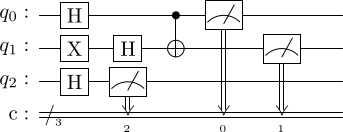
\includegraphics[width=0.72\textwidth]{../figuras/ibm_visualize_circuits_latex.png}
    \caption{Exemplo de circuito quântico com portas \(H\), \(X\), CNOT e operações de medição, apresentado na documentação da IBM Quantum sobre visualização de circuitos no Qiskit. Fonte: IBM Quantum \cite{ibmQuantumVisualizeCircuits2026}.}
    \label{fig:ibm_visualizacao_circuito}
\end{figure}

Para um sistema com \(n\) qubits, o estado quântico pertence a um espaço de dimensão \(2^n\). Por exemplo, dois qubits possuem quatro estados base:

\[
\ket{00}, \ket{01}, \ket{10}, \ket{11}.
\]

De forma geral, um estado de dois qubits pode ser representado por:

\[
\ket{\psi} =
\alpha_{00}\ket{00}
+
\alpha_{01}\ket{01}
+
\alpha_{10}\ket{10}
+
\alpha_{11}\ket{11},
\]

com a condição:

\[
|\alpha_{00}|^2 +
|\alpha_{01}|^2 +
|\alpha_{10}|^2 +
|\alpha_{11}|^2 = 1.
\]

Esse crescimento exponencial do espaço de estados é uma das razões pelas quais a computação quântica desperta interesse em problemas de alta complexidade. Entretanto, esse mesmo crescimento também torna a simulação clássica de circuitos quânticos rapidamente custosa.

Outro fenômeno importante é o emaranhamento. Um estado é dito emaranhado quando não pode ser decomposto como produto tensorial de estados individuais dos qubits. Um exemplo clássico é o estado de Bell:

\[
\ket{\Phi^+} =
\frac{1}{\sqrt{2}}
(\ket{00} + \ket{11}).
\]

Nesse caso, os qubits apresentam correlações que não podem ser descritas apenas como estados independentes. A medição de um qubit afeta a descrição do estado global do sistema, produzindo correlações probabilísticas fortes entre os resultados.

A medição é o processo que transforma informação quântica em informação clássica. Em modelos de aprendizado de máquina quântico, as medições são fundamentais, pois as saídas do circuito geralmente são obtidas por probabilidades de medição ou por valores esperados de observáveis. Por exemplo, pode-se medir o valor esperado do operador de Pauli-Z em um qubit:

\[
\langle Z \rangle =
\bra{\psi} Z \ket{\psi}.
\]

Esse valor esperado pode ser utilizado como uma característica numérica de saída do circuito quântico e, posteriormente, alimentar uma camada clássica de classificação.

\subsection{Portas e circuitos quânticos parametrizados}

As portas quânticas são operações matemáticas aplicadas sobre qubits. Diferentemente de muitas operações clássicas, as portas quânticas são representadas por matrizes unitárias, isto é, matrizes \(U\) que satisfazem:

\[
U^\dagger U = I,
\]

em que \(U^\dagger\) representa a conjugada transposta de \(U\) e \(I\) é a matriz identidade. Essa propriedade garante que a norma do estado quântico seja preservada durante a evolução do circuito.

Entre as portas quânticas mais comuns estão as portas de Pauli \(X\), \(Y\) e \(Z\), a porta Hadamard \(H\), portas de rotação e portas controladas, como CNOT e CZ. A porta Hadamard, por exemplo, é frequentemente utilizada para criar superposição:

\[
H\ket{0} =
\frac{1}{\sqrt{2}}
(\ket{0} + \ket{1}).
\]

Portas de rotação são especialmente importantes em modelos variacionais, pois dependem de parâmetros ajustáveis. Uma rotação em torno do eixo \(Y\), por exemplo, pode ser representada por:

\[
R_Y(\theta) =
e^{-i\frac{\theta}{2}Y}.
\]

De modo geral, um circuito quântico parametrizado pode ser representado por uma operação unitária \(U(\theta)\), em que \(\theta\) representa um conjunto de parâmetros treináveis. Um circuito formado por várias camadas pode ser escrito como:

\[
U(\theta) =
U_L(\theta_L)
U_{L-1}(\theta_{L-1})
\cdots
U_1(\theta_1).
\]

Essa estrutura é análoga, em certo sentido, às redes neurais clássicas, nas quais diferentes camadas aplicam transformações sucessivas aos dados. No caso quântico, as transformações são operações unitárias aplicadas sobre estados quânticos.

Em modelos híbridos, os parâmetros do circuito são ajustados por um otimizador clássico. O circuito quântico calcula uma saída, normalmente associada a valores esperados de observáveis, e essa saída é usada para computar uma função de custo. Em seguida, um algoritmo clássico atualiza os parâmetros do circuito. Esse ciclo forma a base dos algoritmos variacionais quânticos \cite{cerezo2021variational}.

\subsection{Codificação de dados clássicos em estados quânticos}

Para que dados clássicos sejam processados por um circuito quântico, é necessário convertê-los em estados quânticos ou em parâmetros de portas quânticas. Esse processo é chamado de codificação, incorporação ou \textit{embedding} dos dados. A escolha da codificação é uma etapa central em QML, pois determina como a informação clássica será representada no espaço quântico.

Uma forma simples de codificação é a codificação por ângulo. Nesse caso, os atributos clássicos de uma entrada \(x = [x_1, x_2, \ldots, x_d]\) são usados como ângulos de rotação em portas quânticas. Por exemplo, pode-se aplicar uma rotação em cada qubit:

\[
\ket{\psi(x)}
=
\prod_{j=1}^{d}
R_Y(x_j)
\ket{0}^{\otimes n}.
\]

Essa estratégia é simples e adequada para circuitos rasos, mas exige que a dimensão dos dados seja compatível com o número de qubits ou com o número de portas utilizadas. Em imagens de alta dimensão, como mamografias, esse ponto se torna crítico, pois a quantidade de pixels é muito maior do que o número de qubits disponível em dispositivos atuais.

Outra abordagem é o uso de \textit{quantum feature maps}. Nesse caso, os dados clássicos são mapeados para estados quânticos por meio de um circuito \(U_{\Phi}(x)\), produzindo:

\[
\ket{\Phi(x)} =
U_{\Phi}(x)\ket{0}^{\otimes n}.
\]

A motivação é que o espaço de Hilbert pode atuar como um espaço de características de alta dimensão. Havlíček et al. propuseram métodos de aprendizado supervisionado com espaços de características quânticos, incluindo classificadores variacionais e estimadores de kernel quântico. A ideia central é mapear os dados clássicos de forma não linear para estados quânticos e explorar produtos internos nesse espaço para realizar classificação \cite{havlicek2019supervised}.

Em métodos baseados em kernel, a similaridade entre duas entradas \(x\) e \(z\) pode ser calculada por:

\[
K(x,z) =
|\langle \Phi(x) | \Phi(z) \rangle|^2.
\]

Essa formulação estabelece uma conexão direta entre QML e métodos clássicos como SVMs, nos quais a escolha do kernel influencia fortemente a capacidade de separação entre classes.

Uma limitação relevante da codificação é que dados clássicos não podem ser simplesmente copiados dentro de um circuito quântico como ocorre em redes neurais clássicas. Para contornar parte dessa limitação, Pérez-Salinas et al. propuseram a técnica de \textit{data re-uploading}, na qual os mesmos dados clássicos são inseridos repetidas vezes ao longo do circuito. Um circuito com reenvio de dados pode ser representado de forma simplificada como:

\[
U(\theta, x)
=
L_N(\theta_N, x)
\cdots
L_2(\theta_2, x)
L_1(\theta_1, x),
\]

em que cada camada \(L_i\) combina parâmetros treináveis e dados de entrada. Essa técnica aumenta a capacidade expressiva do circuito, permitindo que modelos com poucos qubits representem funções mais complexas \cite{perezsalinas2020data}.

No contexto de imagens médicas, a codificação é um dos maiores desafios para modelos quânticos. Uma mamografia redimensionada para \(1024 \times 1024\) pixels possui mais de um milhão de valores de intensidade, enquanto circuitos quânticos simuláveis geralmente utilizam poucos qubits. Por isso, modelos híbridos normalmente utilizam uma etapa clássica de extração ou compressão de características antes da codificação quântica.

\begin{figure}[H]
    \centering
    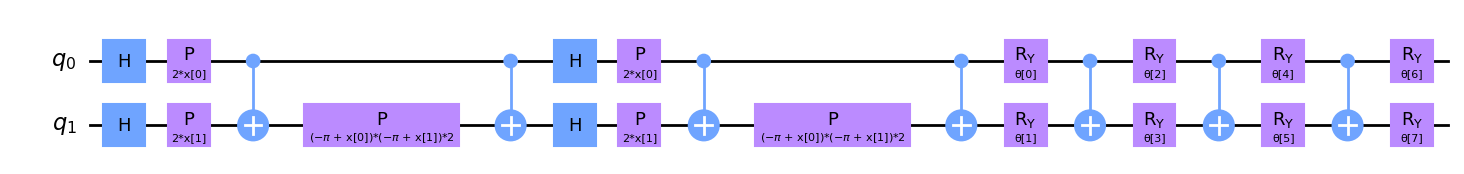
\includegraphics[width=\textwidth]{../figuras/qiskit_ml_torch_connector_qnn_circuit.png}
    \caption{Exemplo de circuito usado em um modelo híbrido no Qiskit Machine Learning, combinando um \textit{feature map} para codificação dos dados com um \textit{ansatz} parametrizado. Fonte: Qiskit Machine Learning \cite{qiskitMachineLearningTorchConnector2026}.}
    \label{fig:qiskit_ml_feature_map_ansatz}
\end{figure}

Além das codificações usadas diretamente em QML, também existem representações quânticas específicas para imagens. Métodos como Qubit Lattice, FRQI e NEQR buscam representar posição e intensidade dos pixels por meio de estados quânticos, amplitudes, ângulos ou registradores binários. Esses modelos ajudam a compreender os desafios de medição e escalabilidade quando se tenta representar imagens em circuitos quânticos \cite{okada2025measurementlimits}.

\subsection{Modelos variacionais quânticos}

Modelos variacionais quânticos são uma das principais abordagens para uso de computação quântica em dispositivos NISQ. Esses modelos combinam circuitos quânticos parametrizados com otimizadores clássicos. O circuito quântico é responsável por preparar estados, aplicar transformações e produzir medições; o computador clássico calcula a função de custo e atualiza os parâmetros do circuito.

A estrutura geral de um algoritmo variacional pode ser descrita por três componentes: uma função de custo \(C(\theta)\), um circuito parametrizado, também chamado de \textit{ansatz}, e um otimizador clássico. O objetivo é encontrar os parâmetros:

\[
\theta^* =
\arg\min_{\theta}
C(\theta).
\]

A função de custo pode depender de medições realizadas no circuito quântico. Em muitos casos, ela pode ser expressa em termos de valores esperados de observáveis:

\[
C(\theta)
=
\sum_k
f_k
\left(
\operatorname{Tr}
[
O_k U(\theta)\rho_k U^\dagger(\theta)
]
\right),
\]

em que \(O_k\) representa um observável, \(\rho_k\) representa um estado de entrada e \(U(\theta)\) é o circuito parametrizado. Essa formulação mostra como o circuito quântico e o otimizador clássico atuam em conjunto no processo de aprendizagem \cite{cerezo2021variational}.

Em classificação, o circuito pode receber uma entrada codificada \(x\), aplicar uma transformação variacional e produzir saídas por medição. Por exemplo:

\[
z_j(x,\theta)
=
\langle Z_j \rangle
=
\bra{\psi(x,\theta)}
Z_j
\ket{\psi(x,\theta)}.
\]

O vetor \(z(x,\theta)\) pode ser utilizado diretamente para classificação ou enviado a uma camada clássica, como uma camada densa com ativação \textit{softmax}. Assim, o circuito quântico atua como uma camada treinável dentro de um pipeline maior.

\begin{figure}[H]
    \centering
    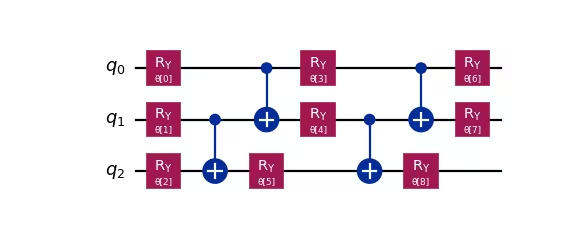
\includegraphics[width=0.78\textwidth]{../figuras/ibm_real_amplitudes_1.png}
    \caption{Circuito \textit{real amplitudes} com camadas de rotações \(R_Y\) e portas CNOT, usado como exemplo de \textit{ansatz} parametrizado na documentação do Qiskit. Fonte: IBM Quantum \cite{ibmQuantumRealAmplitudes2026}.}
    \label{fig:ibm_real_amplitudes}
\end{figure}

A escolha do ansatz é uma decisão importante. Um ansatz muito simples pode não ter capacidade suficiente para representar padrões complexos; por outro lado, um ansatz muito profundo pode ser difícil de treinar e mais sensível a ruído. Essa tensão entre expressividade, profundidade, número de qubits e treinabilidade é uma das principais questões em modelos variacionais quânticos.

\subsection{Limitações NISQ, simulação, barren plateaus e escalabilidade}

Apesar do potencial dos modelos quânticos, sua aplicação prática ainda enfrenta limitações importantes. A primeira delas é o custo de simulação. Um sistema com \(n\) qubits possui \(2^n\) amplitudes complexas. Assim, a memória necessária para simular exatamente um estado quântico cresce exponencialmente com o número de qubits. Essa limitação é especialmente relevante em pesquisas executadas em computadores clássicos, nas quais o aumento do número de qubits rapidamente se torna inviável.

Outro desafio é a presença de \textit{barren plateaus}. Esse termo descreve regiões da paisagem de otimização nas quais os gradientes da função de custo se tornam muito pequenos. Quando isso ocorre, o otimizador clássico tem dificuldade para encontrar direções úteis de atualização dos parâmetros. McClean et al. demonstraram que, para certas famílias de circuitos quânticos parametrizados, a variância dos gradientes pode decair exponencialmente com o número de qubits \cite{mcclean2018barren}.

De forma simplificada, se \(E(\theta)\) representa uma função de custo, o treinamento depende de gradientes como:

\[
\frac{\partial E(\theta)}{\partial \theta_k}.
\]

Em um \textit{barren plateau}, esses gradientes se aproximam de zero para grande parte do espaço de parâmetros:

\[
\frac{\partial E(\theta)}{\partial \theta_k}
\approx 0.
\]

Isso dificulta o treinamento, pois as atualizações de parâmetros tornam-se pouco informativas. Em contraste com redes neurais clássicas, nas quais o desaparecimento do gradiente costuma estar fortemente associado à profundidade da rede, em circuitos quânticos o problema também pode depender fortemente do número de qubits e da forma do ansatz.

A escalabilidade também é limitada pelo ruído dos dispositivos NISQ. Circuitos mais profundos tendem a acumular mais erros, e circuitos com muitos qubits exigem maior conectividade e controle físico. Por isso, modelos híbridos atuais costumam utilizar poucos qubits e circuitos relativamente rasos. Essa escolha melhora a viabilidade prática, mas também pode limitar a expressividade do componente quântico.

Em imagens médicas de alta dimensão, como mamografias, essas limitações são ainda mais evidentes. A codificação direta de todos os pixels é impraticável nos dispositivos atuais, exigindo redução dimensional, extração de características ou processamento local. Portanto, qualquer comparação entre modelos clássicos e híbridos deve considerar não apenas métricas preditivas, mas também custo computacional, estabilidade do treinamento, uso de memória e viabilidade de simulação.

\subsection{Simulação de circuitos quânticos e uso do Qiskit}
\label{subsec:simulacao_circuitos_qiskit}

Como este trabalho será desenvolvido em ambiente clássico, os circuitos quânticos serão avaliados por simulação. Essa escolha permite construir, testar e comparar circuitos parametrizados sem depender de acesso contínuo a hardware quântico real, mas impõe limites práticos de memória, tempo de execução, número de qubits e profundidade dos circuitos.

O Qiskit será utilizado como ferramenta de apoio para a construção e simulação dos circuitos quânticos variacionais. Em especial, simuladores como o Qiskit Aer são relevantes para estudos experimentais porque permitem executar circuitos com controle sobre número de \textit{shots}, medições, estados simulados e custo computacional. A documentação da IBM Quantum descreve o uso do Qiskit Aer com primitivas como \textit{Estimator} e \textit{Sampler}, incluindo simulações exatas e ruidosas \cite{ibmQuantumAerSimulation2026}. Estudos recentes também discutem fluxos híbridos quântico-clássicos e aceleração por GPU em simulações quânticas, incluindo o uso de ferramentas como cuQuantum \cite{faj2023warpspeed,chen2024quantumhpcworkflow,bayraktar2023cuquantum}.

No contexto deste trabalho, o cuQuantum deve ser entendido como uma possibilidade de aceleração da simulação clássica dos circuitos quânticos em GPUs NVIDIA, e não como uma mudança na formulação matemática do modelo híbrido. A Figura~\ref{fig:qiskit_aer_cuquantum_workflow} ilustra esse papel no fluxo do Qiskit Aer: o circuito é otimizado pelo transpilador, executado pelo simulador de vetor de estado e pode usar diferentes backends, incluindo CPU, GPU com Thrust e GPU com cuQuantum.

\begin{figure}[H]
    \centering
    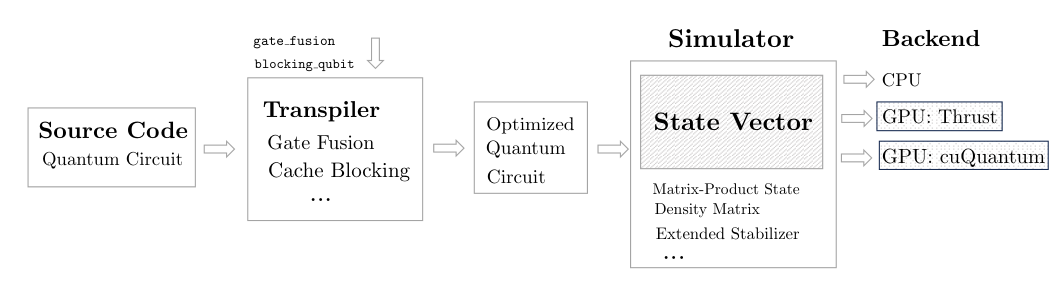
\includegraphics[width=\textwidth]{../figuras/qiskit_aer_cuquantum_workflow_faj2023.png}
    \caption{Fluxo de simulação de vetor de estado no Qiskit Aer, incluindo backends CPU, GPU com Thrust e GPU com cuQuantum. Fonte: extraído de Faj et al. \cite{faj2023warpspeed}.}
    \label{fig:qiskit_aer_cuquantum_workflow}
\end{figure}

Ainda assim, os resultados obtidos por simulação devem ser interpretados com cautela, pois podem não refletir integralmente ruído, conectividade, calibração e restrições operacionais de dispositivos NISQ reais.


\section{Modelos híbridos quântico-clássicos}

Modelos híbridos quântico-clássicos combinam componentes de aprendizado de máquina clássico com circuitos quânticos parametrizados. Essa abordagem é adequada ao cenário NISQ porque permite utilizar circuitos pequenos, enquanto delega ao computador clássico tarefas como pré-processamento, extração de características, otimização e classificação final.

Em tarefas de classificação de imagens, uma estratégia comum é usar uma rede neural clássica, especialmente uma CNN, para extrair características visuais da imagem. Em seguida, essas características são projetadas para uma dimensão compatível com o número de qubits e codificadas em um circuito quântico. O circuito atua como uma camada variacional ou transformadora, e suas saídas são processadas por camadas clássicas responsáveis pela classificação final.

Essa estrutura permite investigar se o componente quântico contribui para a representação dos dados ou para a separação entre classes. No entanto, a simples inclusão de um circuito quântico não garante ganho de desempenho. A contribuição do bloco quântico precisa ser avaliada de forma controlada, comparando-o com baselines clássicos equivalentes.
Essa integração entre redes neurais clássicas e componentes quânticos também aparece na documentação do Qiskit Machine Learning, que exemplifica o uso do \textit{TorchConnector} para incorporar uma rede neural quântica a um fluxo de treinamento em PyTorch \cite{qiskitMachineLearningTorchConnector2026}.

\subsection{Arquitetura híbrida CNN--circuito quântico}

Em um modelo híbrido para classificação, o fluxo geral pode ser descrito por quatro etapas. A primeira é o processamento clássico da entrada. Considerando uma imagem \(x\), uma rede clássica \(g_{\phi}\) pode extrair um vetor de características:

\[
v = g_{\phi}(x),
\]

em que \(\phi\) representa os parâmetros da rede clássica. Em seguida, esse vetor é projetado para uma dimensão menor, compatível com o número de qubits:

\[
u = Wv + b.
\]

\subsection{Camada de codificação clássico-quântica}
\label{subsec:camada_codificacao_classico_quantica}

O vetor \(u\) é então codificado em um circuito quântico por meio de um operador de codificação \(U_{\text{enc}}(u)\), produzindo um estado:

\[
\ket{\psi(u)}
=
U_{\text{enc}}(u)
\ket{0}^{\otimes n}.
\]

\subsection{Camada quântica variacional}
\label{subsec:camada_quantica_variacional}

Depois, aplica-se um circuito variacional \(U(\theta)\), cujos parâmetros são treináveis:

\[
\ket{\psi(u,\theta)}
=
U(\theta)
U_{\text{enc}}(u)
\ket{0}^{\otimes n}.
\]

\subsection{Medição do circuito quântico e retorno ao modelo clássico}
\label{subsec:medicao_retorno_modelo_classico}

A saída do circuito pode ser obtida por valores esperados de observáveis, como operadores de Pauli-Z:

\[
z_j =
\bra{\psi(u,\theta)}
Z_j
\ket{\psi(u,\theta)}.
\]

Esses valores formam um vetor \(z\), que pode ser enviado a uma camada clássica final:

\[
\hat{y}
=
\operatorname{softmax}(W_c z + b_c).
\]

Essa formulação mostra que o circuito quântico pode ser interpretado como uma camada intermediária treinável dentro de uma arquitetura maior. Em problemas de classificação, o treinamento busca ajustar tanto parâmetros clássicos quanto parâmetros quânticos, minimizando uma função de perda associada aos rótulos verdadeiros.

Xiang et al. propuseram uma arquitetura híbrida quântico-clássica para diagnóstico de câncer de mama, combinando uma camada convolucional quântica com camadas clássicas totalmente conectadas. No artigo, os autores utilizam bases como GBSG, SEER e WDBC, que são bases diagnósticas/tabulares, e não uma base de mamografias como o Mammo-Bench \cite{xiang2024qccnn}. Ainda assim, o trabalho é relevante por mostrar uma aplicação direta de modelos híbridos no contexto de câncer de mama.

\subsection{CNN com gargalo clássico como baseline de controle}
\label{subsec:cnn_gargalo_baseline}

A CNN com gargalo clássico será utilizada como baseline de controle porque o modelo híbrido precisa reduzir o vetor de características para uma dimensão compatível com o número de qubits. Sem esse controle, uma eventual diferença de desempenho poderia ser causada pela redução dimensional, e não necessariamente pela presença do circuito quântico. Portanto, o gargalo clássico reproduz a etapa de compactação do modelo híbrido, mas substitui a camada quântica por uma transformação clássica treinável.

\subsection{Comparação com a CNN clássica}
\label{subsec:comparacao_cnn_classica}

A comparação com a CNN clássica depende de compreender como a integração entre CNNs e circuitos quânticos pode ocorrer. Uma abordagem é utilizar a CNN como extratora de características e substituir parte das camadas densas finais por uma camada quântica variacional. Nesse caso, a CNN processa a imagem, reduz sua dimensionalidade e envia ao circuito quântico um vetor compacto de características.

Outra abordagem é utilizar camadas quanvolucionais, propostas por Henderson et al. Nessas camadas, regiões locais da imagem são processadas por circuitos quânticos, de forma análoga ao funcionamento de filtros convolucionais clássicos \cite{henderson2020quanvolutional}. Uma região local da imagem, representada por \(u_x\), é codificada em um circuito quântico por uma função \(e\):

\[
i_x = e(u_x).
\]

Em seguida, o circuito quântico \(q\) transforma esse estado:

\[
o_x = q(i_x) = q(e(u_x)).
\]

Por fim, uma função de decodificação \(d\), baseada em medições, transforma a saída quântica em um valor clássico:

\[
f_x = d(o_x) = d(q(e(u_x))).
\]

A transformação completa pode ser representada por:

\[
f_x = Q(u_x, e, q, d).
\]

Esse valor \(f_x\) passa a compor um mapa de características, de forma semelhante à saída de um filtro convolucional clássico. A principal diferença é que a transformação local não é uma simples multiplicação por um kernel clássico, mas sim o resultado de uma codificação, uma evolução quântica e uma medição.

Essa ideia é interessante para imagens porque evita a necessidade de codificar a imagem inteira em um único circuito. Em vez disso, pequenas regiões locais são processadas separadamente, reduzindo a quantidade de qubits necessária. Essa característica torna as camadas quanvolucionais mais compatíveis com dispositivos NISQ. Entretanto, essa abordagem também pode ser computacionalmente custosa, pois o circuito precisa ser executado muitas vezes para processar todas as regiões da imagem.

No contexto de mamografias, a integração entre CNNs e circuitos quânticos precisa considerar a alta resolução das imagens e a importância de regiões pequenas. Uma arquitetura híbrida pode utilizar camadas convolucionais clássicas para extrair padrões visuais, como textura, contraste e forma, e depois aplicar um circuito quântico apenas sobre uma representação compacta. Essa estratégia reduz o custo quântico e torna o treinamento mais viável.

\subsection{Limitações práticas em imagens de alta dimensão}

A aplicação de modelos híbridos quântico-clássicos em imagens médicas de alta dimensão apresenta desafios específicos. O primeiro desafio é a diferença entre a dimensão da imagem e a quantidade de qubits disponível. Uma mamografia em escala de cinza com resolução \(1024 \times 1024\) possui \(1.048.576\) pixels. Codificar diretamente todos esses valores em um circuito quântico é impraticável nos dispositivos atuais e também em simuladores clássicos.

Por isso, modelos híbridos dependem de alguma forma de compressão, extração de características ou processamento local. Essa redução dimensional, entretanto, pode causar perda de informações relevantes. Em mamografias, lesões pequenas, microcalcificações e alterações sutis podem ocupar regiões muito pequenas da imagem. Assim, se a compressão remover essas informações, o circuito quântico receberá uma representação insuficiente para a classificação.

Outro desafio é o custo de execução. Mesmo circuitos pequenos podem precisar ser avaliados muitas vezes durante o treinamento. Além disso, medições quânticas são probabilísticas, o que pode exigir múltiplas execuções, chamadas de \textit{shots}, para estimar valores esperados com precisão. Em simuladores, o custo cresce com o número de qubits; em hardware real, o custo envolve ruído, tempo de execução e limitações de acesso ao dispositivo.

Também existe o desafio da treinabilidade. Circuitos muito expressivos ou aleatórios podem sofrer com \textit{barren plateaus}, tornando o treinamento instável. Circuitos muito simples, por outro lado, podem não ter capacidade suficiente para separar classes complexas. Dessa forma, há um equilíbrio delicado entre expressividade e treinabilidade.

A revisão de Yan et al. destaca que algoritmos quânticos e quantum-inspired vêm sendo explorados em tarefas de processamento de imagens médicas, incluindo diagnóstico, classificação, segmentação e segurança de imagens. No entanto, os autores também indicam que esse campo ainda apresenta desafios abertos, especialmente devido às limitações da tecnologia quântica atual e à necessidade de validações mais robustas em aplicações reais \cite{yan2024quantumMedicalImageReview}.

Portanto, em imagens de mamografia, modelos híbridos quântico-clássicos devem ser analisados com cautela. A hipótese de que um componente quântico pode melhorar a representação dos dados é relevante do ponto de vista científico, mas precisa ser avaliada por meio de comparações controladas com modelos clássicos. Uma avaliação adequada deve considerar desempenho preditivo, estabilidade, custo computacional, escalabilidade e interpretabilidade. Assim, a contribuição de uma arquitetura híbrida não deve ser assumida previamente, mas investigada experimentalmente.

\section{Trabalhos correlatos}

O câncer de mama é uma doença caracterizada pelo crescimento descontrolado de células mamárias, podendo evoluir para formas invasivas e metastáticas. A Organização Mundial da Saúde ressalta que a mortalidade pode ser reduzida com diagnóstico e tratamento precoces, sendo a mamografia um dos principais instrumentos de rastreamento em populações assintomáticas \cite{WHO2026BreastCancer}. No Brasil, o INCA mantém orientações específicas para o rastreamento mamográfico, o que reforça a relevância da mamografia no contexto nacional \cite{INCA2025Rastreamento}.

No campo computacional, imagens de mamografia são particularmente desafiadoras por apresentarem ruído, variações de contraste, estruturas anatômicas complexas e, em muitos casos, desbalanceamento entre classes. Tais características tornam necessário o uso de métodos robustos de extração de atributos e classificação. Além disso, a definição de mais classes diagnósticas aumenta a dificuldade do problema, exigindo maior cuidado na curadoria dos dados e na avaliação do desempenho.

\subsection{CNNs e aprendizado profundo em mamografia}

O avanço recente da visão computacional está fortemente associado ao desenvolvimento do aprendizado profundo, especialmente com o uso de redes neurais convolucionais. Conforme discutido por \citeonline{LeCun2015}, redes profundas aprendem representações hierárquicas diretamente a partir dos dados, dispensando parte da engenharia manual de atributos tradicional.

Em aplicações médicas, CNNs têm sido empregadas para classificação, detecção e segmentação de padrões em exames de imagem. Na área de mamografia, revisões sistemáticas indicam amplo uso dessas arquiteturas, porém alertam para dificuldades de reprodutibilidade, viés de seleção e falta de avaliação em ambientes mais próximos da prática clínica \cite{Bhalla2023MammographyReview}. Esses pontos justificam a adoção de um protocolo experimental rigoroso neste TCC.

\subsection{Modelos híbridos quântico-clássicos em classificação}

A computação quântica explora propriedades como superposição, emaranhamento e interferência para processamento de informação. Em aprendizado de máquina, uma das linhas mais promissoras tem sido a construção de modelos híbridos, nos quais etapas clássicas e quânticas são combinadas para aproveitar, ao menos em tese, diferentes capacidades de representação.

\subsection{Modelos quânticos e híbridos em imagens médicas}

Entretanto, a literatura recente sugere cautela. A revisão sistemática de \citeonline{Gupta2025QMLDigitalHealth} mostra que, em saúde digital, a maioria dos estudos ainda opera com fortes simplificações, pequeno porte de dados e escopo experimental reduzido. Já \citeonline{long2025qcqcnn} apresenta uma arquitetura híbrida quântico-clássico-quântica com resultados competitivos em bases de imagens e tumores por ressonância magnética, evidenciando potencial, mas também dependência de cenários controlados.

Assim, a comparação entre uma CNN clássica e uma arquitetura híbrida em mamografias torna-se um recorte adequado para investigar, de forma mais controlada, o real benefício dessas abordagens.

\subsection{Comparação entre os trabalhos relacionados}

De modo geral, os trabalhos correlatos indicam que CNNs já constituem uma abordagem consolidada para análise de mamografias, mas ainda enfrentam desafios de reprodutibilidade, validação externa, desbalanceamento e interpretação dos resultados. Em paralelo, modelos quânticos e híbridos apresentam potencial exploratório, porém ainda são avaliados majoritariamente em cenários controlados, bases menores ou tarefas simplificadas.

Essa comparação evidencia a lacuna que orienta este TCC: avaliar, sob o mesmo protocolo experimental, uma CNN clássica, uma CNN com gargalo clássico e uma arquitetura híbrida quântico-clássica simulada em uma base de mamografias. Assim, a contribuição esperada não é assumir superioridade do modelo híbrido, mas verificar de forma controlada se ele apresenta ganhos, perdas ou limitações relevantes em desempenho, custo computacional e estabilidade.


% ---------------------------------------------------------------
% CAPÍTULO 3 - DESENVOLVIMENTO / PROPOSTA METODOLÓGICA
% ---------------------------------------------------------------
\chapter{Desenvolvimento: proposta metodológica}
\label{cap:desenvolvimento}

Neste capítulo, apresenta-se a proposta de desenvolvimento do trabalho a ser realizada no TCC2. Diferentemente de um sistema computacional tradicional, a solução proposta neste trabalho consiste em um pipeline experimental para comparação entre arquiteturas de aprendizado de máquina aplicadas à classificação de mamografias.

O desenvolvimento será conduzido como um estudo experimental comparativo, quantitativo e reprodutível. A proposta consiste em implementar, treinar e avaliar uma rede neural convolucional clássica e uma arquitetura híbrida quântico-clássica simulada, utilizando a mesma base de dados, o mesmo pré-processamento, a mesma divisão entre treino, validação e teste e o mesmo conjunto de métricas. Dessa forma, busca-se realizar uma comparação controlada entre os modelos, considerando não apenas desempenho preditivo, mas também custo computacional, estabilidade e limitações práticas de simulação.

O objetivo do desenvolvimento não é criar uma ferramenta clínica de diagnóstico, nem substituir especialistas da área médica. O trabalho deve ser entendido como uma investigação experimental de viabilidade tecnológica, voltada a analisar se a inserção de um componente quântico simulado em uma arquitetura de classificação de mamografias pode apresentar comportamento competitivo em relação a uma CNN clássica.

% ---------------------------------------------------------------
\section{Solução proposta}
\label{sec:solucao}

A solução proposta consiste no desenvolvimento de um pipeline computacional para classificação supervisionada de mamografias em três classes: normal, benigno e maligno. Esse pipeline será composto por etapas de organização da base de dados, pré-processamento das imagens, definição dos conjuntos de treino, validação e teste, implementação dos modelos, treinamento, avaliação por métricas preditivas e comparação do custo computacional.

A comparação será realizada entre três arquiteturas principais. A primeira será uma CNN clássica, utilizada como modelo de referência. A segunda será uma CNN com gargalo clássico equivalente, cuja função será servir como controle experimental para avaliar o impacto da redução dimensional antes da classificação. A terceira será uma arquitetura híbrida quântico-clássica, composta por uma etapa clássica de extração de características, uma etapa de projeção dimensional e um circuito quântico variacional simulado.

A inclusão de uma CNN com gargalo clássico equivalente é importante porque permite uma comparação mais justa com o modelo híbrido. Caso o modelo híbrido apresente ganho ou perda de desempenho, será possível avaliar se esse comportamento está relacionado ao componente quântico ou apenas à redução dimensional necessária para adaptar os dados clássicos ao número limitado de qubits.

% ---------------------------------------------------------------
\subsection{Visão geral da arquitetura}
\label{subsec:visao_arquitetura}

A arquitetura geral do experimento será organizada em cinco etapas principais:

\begin{enumerate}
    \item seleção e organização da base de dados;
    \item pré-processamento e normalização das imagens;
    \item treinamento da CNN clássica de referência;
    \item treinamento da CNN com gargalo clássico equivalente;
    \item treinamento e avaliação do modelo híbrido quântico-clássico.
\end{enumerate}

Na primeira etapa, serão selecionadas as imagens mamográficas utilizadas na tarefa de classificação. Os rótulos serão organizados em três classes: normal, benigno e maligno. Amostras com rótulos ausentes, inconsistentes ou incompatíveis com a tarefa proposta poderão ser removidas, desde que esse critério seja documentado.

Na segunda etapa, as imagens serão redimensionadas, normalizadas e preparadas para entrada nos modelos. O pré-processamento será mantido igual para todas as arquiteturas, a fim de garantir comparabilidade entre os resultados. Sempre que possível, a divisão dos dados buscará evitar vazamento entre treino, validação e teste, especialmente quando houver metadados que permitam identificar imagens pertencentes ao mesmo paciente ou exame.

Após a divisão dos dados, será aplicada uma estratégia de tratamento do desbalanceamento apenas sobre o conjunto de treinamento. A estratégia principal combinará \textit{undersampling} controlado da classe majoritária com \textit{oversampling} das classes minoritárias, preferencialmente associado a aumento de dados em imagens. O objetivo será reduzir o viés de treinamento causado pela diferença entre as quantidades de exemplos por classe, sem modificar artificialmente a distribuição dos conjuntos de validação e teste. Como alternativa ou análise complementar, também poderá ser testado o \textit{cost-sensitive learning}, por meio de pesos por classe na função de perda, sem reamostrar os dados.

Na terceira etapa, será treinada uma CNN clássica para servir como baseline principal. Essa rede será responsável por extrair características espaciais das mamografias por meio de camadas convolucionais, camadas de normalização, funções de ativação, operações de pooling e camadas finais de classificação.

Na quarta etapa, será implementada uma versão clássica com gargalo dimensional equivalente ao número de entradas utilizadas no circuito quântico. Essa arquitetura terá a função de controlar o efeito da redução dimensional, permitindo avaliar se o desempenho do modelo híbrido decorre realmente da camada quântica ou apenas da compactação das características extraídas pela CNN.

Na quinta etapa, será implementado o modelo híbrido quântico-clássico. Esse modelo utilizará uma CNN para extração inicial de características, uma camada clássica para projetar essas características em um vetor de baixa dimensão e um circuito quântico variacional simulado para processamento intermediário. As saídas do circuito serão encaminhadas para camadas clássicas finais responsáveis pela classificação.

% ---------------------------------------------------------------
\subsection{Tecnologias e ferramentas}
\label{subsec:tecnologias}

O desenvolvimento será realizado em linguagem Python, devido à ampla disponibilidade de bibliotecas para aprendizado profundo, processamento de imagens, análise de dados e computação quântica simulada.

Para a implementação dos modelos clássicos, serão utilizadas bibliotecas como TensorFlow e Keras. Para a manipulação dos dados, organização dos rótulos e análise tabular, serão utilizadas bibliotecas como Pandas e NumPy. Para o cálculo das métricas de avaliação, poderá ser utilizada a biblioteca Scikit-learn. Para geração de gráficos e visualizações, serão utilizadas bibliotecas como Matplotlib.

A parte quântica do trabalho será desenvolvida com apoio do Qiskit, utilizado para a construção e simulação dos circuitos quânticos variacionais. Como o trabalho será realizado em ambiente de simulação, o número de qubits e a profundidade dos circuitos serão limitados pela capacidade computacional disponível.

O ambiente computacional utilizado nos experimentos será documentado, incluindo processador, memória RAM, placa de vídeo, sistema operacional, versões das bibliotecas e configurações principais. Essa documentação é necessária para permitir maior reprodutibilidade dos resultados.

% ---------------------------------------------------------------
\subsection{Funcionalidades principais do pipeline experimental}
\label{subsec:funcionalidades}

O pipeline experimental proposto deverá realizar as seguintes funções:

\begin{itemize}
    \item carregar e organizar os metadados da base de mamografias;
    \item selecionar as imagens e os rótulos correspondentes às classes normal, benigno e maligno;
    \item aplicar o mesmo pré-processamento para todos os modelos;
    \item dividir os dados em treino, validação e teste;
    \item aplicar tratamento do desbalanceamento apenas no conjunto de treinamento, combinando \textit{undersampling} controlado, \textit{oversampling} e, se pertinente, ponderação por custo;
    \item treinar a CNN clássica de referência;
    \item treinar a CNN com gargalo clássico equivalente;
    \item treinar o modelo híbrido quântico-clássico;
    \item registrar histórico de treinamento, perdas e métricas por época;
    \item calcular matriz de confusão, precisão, recall, F1-score e AUC;
    \item comparar tempo de treinamento, uso de memória e estabilidade dos modelos;
    \item gerar tabelas e gráficos para análise dos resultados.
\end{itemize}

Essas funcionalidades permitirão avaliar não apenas qual modelo apresenta melhor desempenho preditivo, mas também qual deles possui melhor viabilidade prática considerando custo computacional, estabilidade e escalabilidade.

% ---------------------------------------------------------------
\subsection{Metodologia de desenvolvimento}
\label{subsec:metodologia_desenvolvimento}

A metodologia de desenvolvimento será dividida em etapas incrementais. Inicialmente, será consolidado o pipeline de dados, garantindo que as imagens sejam carregadas corretamente, os rótulos estejam consistentes e os conjuntos de treino, validação e teste estejam definidos. Em seguida, será implementada a CNN clássica de referência, que servirá como baseline principal do estudo.

Após a definição do baseline clássico, será implementado o modelo clássico com gargalo dimensional equivalente. Esse modelo será utilizado como controle metodológico, pois terá uma redução dimensional semelhante àquela necessária para alimentar o circuito quântico, porém sem utilizar uma camada quântica.

Em seguida, será implementado o modelo híbrido quântico-clássico. Nessa etapa, serão testadas configurações limitadas de número de qubits, profundidade do circuito, estratégia de codificação dos dados e tipo de circuito variacional. Como a simulação quântica possui custo computacional elevado, os experimentos serão planejados de forma progressiva, iniciando com configurações menores e aumentando a complexidade apenas quando houver viabilidade de execução.

Todos os modelos serão avaliados sob o mesmo protocolo experimental. A seleção do melhor modelo será realizada com base no conjunto de validação, enquanto o conjunto de teste será reservado para a avaliação final. Sempre que possível, os experimentos serão repetidos com diferentes sementes aleatórias, permitindo avaliar a estabilidade dos resultados.

% ---------------------------------------------------------------
\subsection{Critérios de validação}
\label{subsec:criterios_validacao}

A validação da solução será realizada por meio da comparação entre os modelos implementados. As métricas principais serão AUC macro, F1-score macro e recall da classe maligna. A acurácia também será registrada, mas será tratada como métrica complementar, pois pode ser influenciada pelo desbalanceamento entre as classes.

A matriz de confusão será utilizada para analisar os tipos de erro cometidos por cada modelo, especialmente os falsos negativos da classe maligna. Esse ponto é importante porque, em tarefas relacionadas à classificação de imagens médicas, erros envolvendo a classe maligna possuem maior relevância crítica.

O conjunto de validação será utilizado para acompanhar o treinamento, selecionar hiperparâmetros e comparar configurações sem acessar o conjunto de teste. Embora a validação possa ser estratificada para preservar a proporção das classes, ela não será balanceada artificialmente por reamostragem, pois isso poderia induzir escolhas de hiperparâmetros ajustadas a uma distribuição diferente da condição real de uso. O conjunto de teste, por sua vez, será mantido sem balanceamento artificial e utilizado apenas ao final, de modo que as métricas finais reflitam a distribuição original dos dados. Análises complementares com subconjuntos balanceados poderão ser relatadas apenas como diagnóstico adicional, não como resultado principal.

Além das métricas preditivas, serão avaliados critérios computacionais, como tempo de treinamento, tempo de inferência, uso de memória, estabilidade entre execuções e limitações de escalabilidade. No caso do modelo híbrido, também serão analisados os impactos do número de qubits, da profundidade do circuito e da estratégia de codificação dos dados clássicos.

A comparação entre os modelos não terá como objetivo demonstrar superioridade prévia da abordagem híbrida. O foco será analisar, sob o mesmo protocolo experimental, como a CNN clássica, a CNN com gargalo clássico e o modelo híbrido quântico-clássico se comportam em métricas preditivas, custo computacional, estabilidade e limitações de simulação. Caso o modelo híbrido apresente desempenho inferior, custo elevado ou dificuldade de convergência, esses resultados também serão considerados relevantes, pois contribuirão para compreender as limitações práticas da abordagem híbrida quântico-clássica nesse tipo de problema.

% ---------------------------------------------------------------
\section{Cronograma de trabalho}
\label{sec:cronograma}

O cronograma a seguir apresenta as atividades previstas para o desenvolvimento do TCC2, distribuídas ao longo de dezesseis semanas. As etapas foram organizadas de modo a contemplar a revisão dos fundamentos teóricos, a preparação dos dados, a implementação dos modelos, a execução dos experimentos, a análise dos resultados e a redação final do trabalho.

\begin{figure}[htb]
    \centering
    \caption{Cronograma de atividades -- Diagrama de Gantt}
    \label{fig:gantt}
    \resizebox{\textwidth}{!}{%
    \begin{ganttchart}[
        hgrid,
        vgrid,
        x unit=0.72cm,
        y unit title=0.6cm,
        y unit chart=0.7cm,
        title height=1,
        bar height=0.5,
        bar label font=\scriptsize,
        title label font=\small,
        milestone label font=\scriptsize\itshape,
        group label font=\scriptsize\bfseries,
        bar/.append style={fill=blue!40},
        group/.append style={draw=black, fill=blue!70},
        milestone/.append style={fill=red!70},
    ]{1}{16}

        \gantttitle{Semanas}{16} \\
        \gantttitlelist{1,...,16}{1} \\

        \ganttgroup{Fase 1: Revisão e planejamento}{1}{3} \\
        \ganttbar{Ajuste da fundamentação teórica}{1}{2} \\
        \ganttbar{Definição final do protocolo experimental}{2}{3} \\
        \ganttmilestone{Protocolo definido}{3} \\

        \ganttgroup{Fase 2: Preparação dos dados}{4}{6} \\
        \ganttbar{Organização da base e rótulos}{4}{5} \\
        \ganttbar{Pré-processamento das imagens}{5}{6} \\
        \ganttbar{Divisão em treino, validação e teste}{6}{6} \\
        \ganttmilestone{Base preparada}{6} \\

        \ganttgroup{Fase 3: Implementação dos modelos}{7}{10} \\
        \ganttbar{Implementação da CNN clássica}{7}{8} \\
        \ganttbar{Implementação do baseline com gargalo}{8}{9} \\
        \ganttbar{Implementação do modelo híbrido}{9}{10} \\
        \ganttmilestone{Modelos implementados}{10} \\

        \ganttgroup{Fase 4: Experimentos e análise}{11}{14} \\
        \ganttbar{Treinamento e ajuste dos modelos}{11}{12} \\
        \ganttbar{Execução dos testes comparativos}{12}{13} \\
        \ganttbar{Análise das métricas e gráficos}{13}{14} \\
        \ganttmilestone{Resultados analisados}{14} \\

        \ganttgroup{Fase 5: Redação e finalização}{13}{16} \\
        \ganttbar{Redação dos resultados}{13}{15} \\
        \ganttbar{Revisão final do texto}{15}{16} \\
        \ganttbar{Preparação da apresentação}{15}{16} \\
        \ganttmilestone{Entrega final}{16}

    \end{ganttchart}%
    }
    \legend{Fonte: Elaborado pelo autor.}
\end{figure}


% ---------------------------------------------------------------
% ELEMENTOS PÓS-TEXTUAIS
% ---------------------------------------------------------------
\postextual

\bibliography{tcc_math}

\end{document}
